\documentclass{beamer}
\usetheme[secheader]{Madrid}

\usepackage[spanish]{babel}
\usepackage[T1]{fontenc}
\usepackage{amsmath,amssymb}
\usepackage{minted}
\usepackage{bm}
\usepackage{tikz}
\usetikzlibrary{tikzmark, calc, arrows, intersections, decorations.pathreplacing, calligraphy}
\usepackage{pgfplots}
\usepackage{multicol}
\usepackage{graphicx}
\usepackage[svgnames]{xcolor}
\usepackage{mathtools}
\usepackage{pifont}
\usepackage{tcolorbox}
\usepackage{tabularray}
\usepackage{subcaption}
\usepackage{svg}

\setbeamercolor{block title alerted}{bg=Gold!80!Goldenrod, fg=black}
\setbeamercolor{block body alerted}{bg=Gold!20!white, fg=black}

\newcommand{\sfb}[1]{\text{\bfseries\sffamily #1}}

\title[Complejidad y Jueces Online]{Complejidad de Algoritmos y Jueces Online}

\author[Ariel Fideleff]{Ariel Leonardo Fideleff\\[2ex]\scriptsize{}Entrenamiento en Programación Competitiva\\Facultad de Ingeniería - Universidad Nacional de Jujuy (UNJu)}

\date{\\\vspace{-3ex}31 de mayo del 2025}

\beamertemplatenavigationsymbolsempty

\begin{document}
    \frame{\titlepage}

    \begin{frame}
        \tableofcontents
    \end{frame}
    
    \section{Introducción}
    \begin{frame}
        \tableofcontents[currentsection]
    \end{frame}

    \begin{frame}
        \begin{center}
            \Huge
            ¡Hola!
        \end{center}
    \end{frame}

    \section{Complejidad computacional}
    \frame{\tableofcontents[currentsection]}

    \subsection{Un ejemplo}
    \frame{\tableofcontents[currentsection, currentsubsection]}

    \begin{frame}[fragile]{Empecemos por un ejemplo}
        \pause
        Veamos el siguiente código en C++:\vspace{10pt}

        \pause

        \begin{minted}[fontsize=\small]{cpp}
void sort(vector<int> &arr, int n) {
    for (int i = 0; i < n; i++)
        for (int j = i+1; j < n; j++)
            if (arr[j] < arr[i])
                swap(arr[i],arr[j]); // Intercambia los números
}
        \end{minted}

        \pause
        ¿Qué hace? \pause Ordena una lista de enteros de menor a mayor!\vspace{8pt}

        \pause

        En efecto, en cada vuelta del primer \mintinline{cpp}{for}, se elige el elemento más chico entre ese y los que le siguen.\pause
        
        Este algoritmo es conocido, se llama \textbf{selection sort}.
    \end{frame}

    \begin{frame}{Otro algoritmo para la misma cosa}
        Ordenar números es fácil, no? \pause Y tampoco es la única forma... \pause \vspace{8pt}

        \begin{minipage}{.48\linewidth} 
            {\fontsize{4}{5}\selectfont
            \inputminted{cpp}{code/merge_sort1.cpp}
            }
        \end{minipage}
        \begin{minipage}{.48\linewidth}
            \inputminted[fontsize=\tiny]{cpp}{code/merge_sort2.cpp}
        \end{minipage}
        
        \pause

        Mucho código... \pause pero también ordena una lista de enteros de menor a mayor! \pause

        Este algoritmo también es conocido, se llama \textbf{merge sort}.
    \end{frame}

    \begin{frame}[fragile]{La liebre versus la tortuga}
        Pero pará, si \textit{selection sort} ordena una lista, es corto y fácil de entender, ¿para qué usaría \textit{merge sort}? \pause

        Para entenderlo, usaremos el comando \texttt{time} de Linux. \pause

        Supongamos que tenemos una lista aleatoria de $10^5$ enteros... (sí, son muchos enteros) \pause

        \begin{figure}
            \begin{subfigure}[c]{.37\linewidth}
                \centering
                \begin{tcolorbox}[nobeforeafter, top=2pt, right=2pt, bottom=2pt, left=2pt]
                    \begin{minted}[fontsize=\tiny]{shell-session}
[ariel@arch-pve code]$ time ./msort

real    0m0.040s
user    0m0.040s
sys     0m0.000s
                \end{minted}
                \end{tcolorbox}
                \caption{Merge Sort}
            \end{subfigure}\pause
            \quad
            \begin{subfigure}[c]{.37\linewidth}
                \centering
                \begin{tcolorbox}[nobeforeafter, top=2pt, right=2pt, bottom=2pt, left=2pt]
                    \begin{minted}[fontsize=\tiny]{shell-session}
[ariel@arch-pve code]$ time ./ssort

real    0m45.235s
user    0m45.133s
sys     0m0.000s
                \end{minted}
                \end{tcolorbox}
                \caption{Selection Sort}
            \end{subfigure}
        \end{figure} \vspace{-8pt} \pause

        Parece que una de las dos se toma su tiempo. \pause 

        Entonces incluso teniendo dos algoritmos que logran exactamente lo mismo, hay diferencias que van más allá de sus resultados. 
        \pause 

        Al final tanto código sí servía para algo, no?
    \end{frame}

    \subsection{Definición}
    \begin{frame}
        \tableofcontents[currentsection, currentsubsection]
    \end{frame}

    \begin{frame}{$\mathcal{O}$ qué!?}
        En Programación Competitiva nos gusta que las cosas sean rápidas. \pause

        Uno de los desafíos del deporte no es sólo lograr resolver lo que nos piden, sino también rápido (nosotros en pensar, y el programa en computar). \pause

        Así, viene útil poder identificar ``qué tan rápido'' es un programa con mirarlo un poco. \pause 

        Para ello se usa frecuentemente la \textbf{notación $\bm{\mathcal{O}}$}, también llamada \textbf{notación O grande}, \textbf{cota superior asintótica}, o bien como le decimos nosotros ``el programa corre en O en [lo que haya dentro de los paréntesis]''.
    \end{frame}


    \begin{frame}{¿Cómo L$\mathcal{O}$ usamos?}
        Buenísimo entonces, tenemos una herramienta para saber qué tan rápido es un programa. \pause Igual... cómo la usamos? \pause 

        \only<-6>{\vspace{8pt}Consideremos un programa que recibe en su entrada una cantidad de datos $n$. \pause Si a partir de un ``$n$ suficientemente grande'' la cantidad de operaciones que ejecuta el programa es \textbf{a lo sumo} $c * n$, donde $c$ es una constante \textit{positiva}, entonces decimos que corre en $\mathcal{O}(n)$.\vspace{8pt}}
        \only<7->{
            \begin{block}{Definición (notación $\mathcal{O}$, informal)}
            Sea un programa que recibe una cantidad de datos $n$. Si a partir de un $n$ suficientemente grande la cantidad de operaciones que ejecuta es \textbf{a lo sumo} $c * n$, donde $c$ es una constante \textit{positiva}, entonces decimos que el programa corre en $\mathcal{O}(n)$.
            \end{block}
        } \pause

        \only<-5>{Veamos un ejemplo.} \only<6->{Veamos un ejemplo... pero primero reescribamos un poco y enmarquemos la definición de antes para tenerla como referencia.} \only<8->{Ahí va.}
    \end{frame}


    \begin{frame}[fragile]{Un programa que corre en $\mathcal{O}(n)$}
        \begin{block}{Definición (notación $\mathcal{O}$, informal)}
            \small{}Sea un programa que recibe una cantidad de datos $n$. Si a partir de un $n$ suficientemente grande la cantidad de operaciones que ejecuta es \textbf{a lo sumo} $c * n$, donde $c$ es una constante \textit{positiva}, entonces decimos que el programa corre en $\mathcal{O}(n)$.
        \end{block}

        \pause

        \only<-9>{Consideremos un programa que lee los números de una lista y los suma: \vspace{6pt}}

        \pause

        \begin{minted}[fontsize=\scriptsize, escapeinside=??]{cpp}
int arr[1000];
int n; cin >> n;?\tikzmark{readn}?
for (int i = 0; i < n; i++)?\tikzmark{readsum}?
    cin >> arr[i];

int sum = 0;
for (int i = 0; i < n; i++)?\tikzmark{sumsum}?
    sum += arr[i];

cout << sum;?\tikzmark{writesum}?
        \end{minted}

        \only<6-8>{Hicimos entonces $2n$ operaciones. O sea, $c * n$ con $c = 2$} \only<7-8>{... no?}
        \only<9->{Hicimos entonces $2n+2$ operaciones. $2n+2 \leq 2n+n = 3n$ para $n \geq 2$.} 
        \uncover<10->{Por lo tanto, este programa corre en $\mathcal{O}(n)$, pues ejecuta a lo sumo $3n$ operaciones a partir de un $n$ ``suficientemente grande''.}
        \begin{tikzpicture}[remember picture, overlay]
            \uncover<4->{\node at ($(pic cs:readsum) + (3.2,0.08)$) {\small$\rightarrow$ $n$ operaciones (leemos $n$ números)};}
            \uncover<5->{\node at ($(pic cs:sumsum) + (3.4,0.08)$) {\small$\rightarrow$ $n$ operaciones (sumamos $n$ números)};}
            \uncover<8->{
                \alt<8>{\node at ($(pic cs:readn) + (4.4,0.08)$) {\textbf{\scriptsize$\bm{\rightarrow}$ 1 operación (leemos 1 número)}};}
                        {\node at ($(pic cs:readn) + (4.25,0.08)$) {\scriptsize$\rightarrow$ 1 operación (leemos 1 número)};}
            }
            \uncover<8->{
                \alt<8>{\node at ($(pic cs:writesum) + (5.35,0.08)$) {\textbf{\scriptsize$\bm{\rightarrow}$ 1 operación (imprimimos 1 número)}};}
                        {\node at ($(pic cs:writesum) + (5.15,0.08)$) {\scriptsize$\rightarrow$ 1 operación (imprimimos 1 número)};}
            }
        \end{tikzpicture}
    \end{frame}

    \begin{frame}{Definición formal (para los más curiosos)}
        En realidad la notación $\mathcal{O}$ nos permite acotar una función cuando su argumento tiende a infinito. \pause 

        Cuando vimos que el programa ``corría en $\mathcal{O}(n)$'' definimos implícitamente una función $f(n) = 2n+2$ a la cual le atribuímos describir la cantidad de operaciones que ejecuta en función de la entrada. \pause
        \begin{block}{Definición (notación $\mathcal{O}$)}
            Sean funciones $f,g : \mathbb{N} \rightarrow \mathbb{R}$, decimos que $f \in \mathcal{O}(g)$ si $\exists \, c \in \mathbb{R}^+_0, n_0 \in \mathbb{N}$ tal que $0 \leq f(n) \leq c . g(n), \; \forall n \geq n_0$.
        \end{block}

        \pause

        Es decir, si graficáramos ambas funciones $f(n) = 2n+2$ y $g(n) = n$, existe $n_0 = 2$ natural a partir del cual la función $f$ siempre tiene valores menores o iguales que la función $c . g = 3g = 3n$. \pause La función $f$ está \textbf{acotada} por $c . g$.
    \end{frame}

    \subsection{Chau constantes (o casi)}
    \begin{frame}
        \tableofcontents[currentsection, currentsubsection]
    \end{frame}

    \begin{frame}{Una constante no deja de ser constante}
        Como vimos en el ejemplo de la sección anterior, las constantes no afectan a la cota $\mathcal{O}$ de un programa. \pause

        Si bien técnicamente por definición podríamos decir que un programa ``corre en $\mathcal{O}(2n)$'' en vez de decir que corre en $\mathcal{O}(n)$, no tiene mucho sentido hacerlo porque lo que más afecta a la rapidez de nuestro programa para una entrada suficientemente grande es la cantidad de operaciones que realiza respecto a su tamaño. \pause

        \vspace{8pt}

    Podemos pensarlo de la siguiente forma: si el factor constante de nuestro programa que corre en $\mathcal{O}(n)$ es muy alta, por ejemplo $c = 1000$, entonces a partir de $n = 1000$, un programa que corre en $\mathcal{O}(n^2)$ realiza más operaciones que el primero:
    \end{frame}

    \begin{frame}[fragile,noframenumbering]
        \begin{center}
    \begin{tikzpicture}
    \begin{axis}[
        width=7cm, height=7cm,
        xmin=0, xmax=1500,
        ymin=0, ymax=130000,
        axis lines=middle,
        xlabel={$n$},
        ylabel={},
        samples=150,
        domain=0:1500,
        clip=true,
        tick label style={font=\tiny},
        label style={font=\small},
        ytick={0,20000,40000,60000,80000,100000,120000},
        yticklabels={0,200000,400000,600000,800000,1000000,1200000},
        scaled y ticks=false,
        every axis plot/.append style={thick}
    ]

        \only<2->{
        \addplot[blue] {x/10}
            node[pos=0.7, anchor=south west, font=\tiny, text=blue] {$f_1(n) = n$};
        }

        \only<3->{
        \addplot[red] {100*x}
            node[pos=0.7, anchor=west, font=\tiny, text=red] {$f_1'(n) = 1000n$};
        }

        \only<4->{
        \addplot[green!60!black] {x^2/10}
            node[pos=0.55, anchor=north east, font=\tiny, text=green!60!black] {$f_2(n) = n^2$};
        }

    \end{axis}
    \end{tikzpicture}
\end{center}
    \end{frame}

    \begin{frame}{Resolver problemas va más allá de las constantes}
        Así, en la práctica observamos que: \pause
        \begin{itemize}
            \item Normalmente el factor constante de una solución no afecta su correctitud a la hora de ser evaluada.
                \pause
            \item A la hora de comparar potenciales soluciones a un problema, se lo suele hacer sin tener en cuenta las constantes, pues éstas están más sujetas a detalles de la implementación de una solución, que a diferentes ideas para resolver un problema.
                \pause
            \item Reducir el factor constante utilizado por un programa suele tratarse de hacer pequeñas modificaciones al código sin cambiar la idea fundamental de la solución que implementa.
                \pause
            \item Cambios en la complejidad (la cantidad de recursos utilizados por el programa) más significativos que los dados por una constante, suelen estar dados por observaciones más importantes y cambios más profundos a la idea para resolver el problema.
        \end{itemize}

    \end{frame}

    \begin{frame}{Siempre hay un pero}
        Por supuesto, hay excepciones, y puede pasar que en algunos casos el límite de tiempo sea algo ajustado, o cuando una solución tenga un factor de constante muy grande, éste sea factor que pueda decidir entre si una solución es considerada correcta o incorrecta por el sistema automático de evaluación. \pause \vspace{8pt}

        Más aún, en algunos casos muy raros puede ser la intención del/los autor/es de un problema en que reducir la constante sea necesario para resolverlo (investigar \mintinline{cpp}{std::bitset}). \pause \vspace{8pt}

        A pesar de todo esto, la conclusión que se deben llevar es que es bueno saber qué es el factor constante de un programa, pero no es esencial reducirlo para resolver problemas, especialmente cuando uno empieza (en los casos más sencillos hasta el compilador los optimiza auutomáticamente!).
    \end{frame}

    \begin{frame}[fragile]{Los beneficios de ignorar constantes}
        Volviendo al ejemplo anterior de la suma de números, se vuelve más sencillo analizar la cota superior asintótica del programa. \pause \vspace{8pt}

        \begin{minted}[fontsize=\scriptsize, escapeinside=??]{cpp}
int arr[1000];
int n; cin >> n;
for (int i = 0; i < n; i++)?\tikzmark{readsum2}?
    cin >> arr[i];

int sum = 0;
for (int i = 0; i < n; i++)
    sum += arr[i];

cout << sum;
        \end{minted}

        \pause
        \begin{tikzpicture}[remember picture, overlay]
            \node at ($(pic cs:readsum2) + (1.5,0.08)$) {\small$\rightarrow$ $n$ operaciones};
        \end{tikzpicture}

        \pause

        Listo! Como vemos que en ningún otro lugar hacemos más de $n$ operaciones, cualquier otra cantidad de operaciones que contemos será múltiplo de $n$, o bien una constante, los cuales no modificarán la cota $\mathcal{O}$ del programa.
    \end{frame}

    \subsection{Algunos órdenes de complejidad comunes}
    \begin{frame}
        \tableofcontents[currentsection, currentsubsection]
    \end{frame}
    
    \begin{frame}{Decidite con los nombres, ¿cota o \textit{complejidad}?}
        \begin{itemize}
            \item Antes mencionamos al pasar que la complejidad de un programa, normalmente llamado \textbf{complejidad computacional}, es la cantidad de recursos utilizados para correr un programa. \pause

            \item Llamamos \textbf{complejidad asintótica computacional} al uso de \textit{análisis asintótico} (como determinar la cota asintótica $\mathcal{O}$ con la que corre un programa) para estimar la complejidad computacional de un programa. \pause

            \item Otra forma de decir que un programa ``corre en $\mathcal{O}(n)$'' es decir que es del \textbf{orden} $\mathcal{O}(n)$ (formalmente, si $f \in \mathcal{O}(g(x))$, entonces $f(x)$ es del orden de $g(x)$). \pause
        \end{itemize}

        Así, como vimos que las constantes no son relevantes para el análisis de la cota $\mathcal{O}$, existen ciertos \textit{órdenes de complejidad} comunes para los programas que \textbf{no} varían por constantes. \pause Reciben ese nombre porque justamente describen mediante notación $\mathcal{O}$ la complejidad de un programa.  \pause

        Sirven como categorías para decir ``en qué corren'' los programas.
    \end{frame}
    
    \begin{frame}{$\mathcal{O}(1)$}
        Decimos que un programa corre en tiempo \textbf{constante} o simplemente en ``O en 1'', y lo notamos $\mathcal{O}(1)$, si, como dice el nombre, su tiempo de ejecución está dado meramente por un factor constante, que no depende del tamaño de la entrada. \pause \vspace{8pt}

        En Programación Competitiva los problemas cuya solución tiene esta cota asintótica suelen estar dados por cuentas matemáticas, por ejemplo.
    \end{frame}

    \begin{frame}[fragile]{$\mathcal{O}(1)$ (ejemplo)}
        \begin{block}{Problema (\only<1>{Watermelon}\only<2->{Watermelon, \textbf<2,3>{CodeForces 4A\tikzmark{cf}}})}
            \uncover<4->{Pete y Billy quieren dividir una sandía de peso $w$ kg en dos pedazos con peso \textbf{par}. Dado $w$, ¿es posible?}
        \begin{tikzpicture}[remember picture, overlay]
            \node (a) at ($ (pic cs:cf) + (-1.5,-.75) $) {};
            \only<3>{
                \node at (a) {(Juez Online, más adelante)};
                \draw[->, thick] ($ (a) + (0,0.2) $) -- ($ (pic cs:cf) + (-1.5,-.25) $);
            }
        \end{tikzpicture}
        \end{block}
        
        \uncover<5->{En otras palabras, queremos determinar si existen dos números $a$ y $b$ tal que $a+b = w$ y $a,b$ pares.}

        \uncover<6->{La suma de dos números pares siempre es par, entonces $w$ \textbf{debe} ser par.} \vspace{4pt}

        \begin{actionenv}<7->
        \begin{minted}[fontsize=\small, escapeinside=??]{cpp}
int w; cin >> w;?\tikzmark{readw}?
if ((w%2) == 0) ?\tikzmark{evenw}?
    cout << "YES"; ?\tikzmark{writey}?
else
    cout << "NO"; ?\tikzmark{writen}?
        \end{minted}
        \end{actionenv}

        \vspace{4pt}
        \uncover<11->{Todas constantes, corre en $\mathcal{O}(1)$!} \uncover<12->{Hmmm, pero estará bien?}

        \uncover<13->{Más adelante lo probaremos en el \textbf{juez}...}
        
        \begin{tikzpicture}[remember picture, overlay]
            \coordinate (xbase) at ($ (pic cs:readw) + (1.5,0.08) $);
            \coordinate (evenw) at ($ (pic cs:evenw) + (0,0.08) $);
            \coordinate (writey) at ($ (pic cs:writey) + (0,0.08) $);
            \coordinate (writen) at ($ (pic cs:writen) + (0,0.08) $);

            \uncover<8->{
                \node[anchor=west, align=left] (a) at (xbase) {\small$\leftarrow$ 1 operación (leer un número)};
            }
            \uncover<9->{
                \node[anchor=west, align=left] (b) at (xbase |- evenw) {\small$\leftarrow$ 2 operaciones (sacar resto \texttt{\%2} y comparar con 0)};
            }
            \uncover<10->{
                \node[anchor=west, align=left] (c) at (xbase |- writey) {\small$\leftarrow$ 1 operación (imprimir la respuesta)};
                \node[anchor=west, align=left] (d) at (xbase |- writen) {\small$\leftarrow$ 1 operación (imprimir la respuesta)};
            }
        \end{tikzpicture}
    \end{frame}

    \begin{frame}{$\mathcal{O}(log \, n)$}
        En este caso, decimos que un programa corre en tiempo \textbf{logarítmico} o en ``O log n'' (se lee tal cual) si el programa ejecuta $log \, n$ operaciones, dada una entrada de $n$ elementos. \pause 
        \begin{block}{Observación}
            La base del logaritmo \textbf{no importa}. \pause En efecto, $log_a \, n$ y $log_b \, n$ para $a \neq b$ difieren en una \textit{constante}. \pause Por propiedad del logaritmo: \pause

            $$ \frac{log_a \, n}{log_a \, b} = log_b \, n \Rightarrow \pause log_a \, n = \onslide<7-> \underbrace{ \onslide<6-> log_a \, b \onslide<7-> }_{constante} \onslide<6-> \, . \;\; log_b \, n$$
        \end{block}
    \end{frame}

    \begin{frame}{$\mathcal{O}(log \, n)$ (¿ejemplo?)}
        Si nos ponemos a pensar, no es tan fácil que una solución completa a un problema en Programación Competitiva tenga un orden de complejidad $\mathcal{O}(log \, n)$. \pause

        Al fin y al cabo, si tenemos que leer $n$ elementos en la entrada, eso ya nos cuenta $n$ operaciones, y como $n \leq log \, n$ para $n \geq 0$, el programa correrá en al menos $\mathcal{O}(n)$. \pause Incluso si el programa que tenemos que hacer no lee los datos (por ejemplo en OIA), seguramente debamos recorrer todos los datos alguna vez para hacer algo con ellos...\pause.............. \pause \vspace{8pt}

        Analicemos entonces la complejidad de un fragmento de código!
    \end{frame}

    \begin{frame}{$\mathcal{O}(log \, n)$ (¡ejemplo!)}
        \begin{block}{Problema (búsqueda binaria)} 
            \pause
            Dado un arreglo \textbf{ordenado} de $n$ números enteros, queremos buscar el menor número de la lista que sea mayor o igual a un número $x$.
        \end{block} \pause
        Este algoritmo es muy conocido. La solución consiste en aprovechar que el arreglo se encuentra ordenado para descartar la mitad de los números del arreglo en cada paso. \pause 

        \begin{itemize}

            \item Si la mediana del arreglo (\texttt{arr[(n-1)/2]}) es mayor o igual al número $x$, como los elementos en posiciones más grandes son todos mayores, sabemos que el número buscado está en en el intervalo $(-1, \lfloor\frac{n-1}{2}\rfloor]$, descartando los últimos $\lfloor\frac{n}{2}\rfloor$ elementos. \pause 

            \item Análogamente, si su mediana es menor a $x$, como todos los elementos en posiciones más chicas son también menores a $x$, sabemos que el número buscado está en el intervalo $(\lfloor \frac{n-1}{2} \rfloor, n)$, descartando los primeros $\lceil\frac{n}{2}\rceil$ elementos.
        \end{itemize}
    \end{frame}
    
    \begin{frame}[fragile,noframenumbering]
        \begin{minted}[fontsize=\scriptsize,escapeinside=??]{cpp}
int x;
vector<int> arr(n); // Suponemos que está ordenado
// ...
int lo = -1, hi = n;
while (hi-lo > 1) {?\tikzmark{binarycmp}?
    int mid = (hi+lo)/2;?\tikzmark{binaryops1}?
    if (arr[mid] >= x) hi = mid;
    else lo = mid;?\tikzmark{binaryops2}?
}
// El menor número mayor o igual a x está en arr[hi].
// Si no existe, termina con hi = n.
        \end{minted}
        \vspace{4pt}
        \uncover<5->{De esta forma, corre en $\mathcal{O}(log \, n)$! (recordemos que la base del logaritmo no importaba)}
        \vspace{8pt}

        \uncover<6->{En muchas soluciones de Prog. Competitiva se usa binary search \textbf{como parte de la solución}. Incluso es parte de la librería estándar de C++ (ver \mintinline{cpp}{std::lower_bound}).}

        \uncover<7->{Es por esto que también es importante saber analizar la complejidad de ``pedazos de programas'', para luego obtener la cota asintótica $\mathcal{O}$ para la solución completa.}

        \begin{tikzpicture}[remember picture, overlay]
            \coordinate (a) at ($ (pic cs:binarycmp) + (5,0.08) $);
            \coordinate (b) at ($ (pic cs:binaryops1) + (1.25, 0.2) $);
            \coordinate (c') at (pic cs:binaryops2);
            \coordinate (c) at ($ (b |- c') + (0, -0.08) $);
            \onslide<2->{\node[align=left] at (a) {\scriptsize$\leftarrow$ Cada iteración \texttt{hi-lo} se reduce aprox. a la mitad};}
            \onslide<3->{\node[align=center] at ($ (a.south) + (0,-.325) $) {\scriptsize{} (def. logaritmo, $\approx log_2 \, n$ iteraciones)};}
            \onslide<4->{\draw[decorate, decoration={calligraphic brace,amplitude=4pt,aspect=0.7}, line width=1pt] (b) -- (c) node[pos=0.7, right, yshift=.35pt, xshift=4pt] {\scriptsize constante};}
        \end{tikzpicture}
    \end{frame}

    \begin{frame}{$\mathcal{O}(n)$}
        Un programa corre en tiempo \textbf{lineal} o en ``O en n'' si el programa ejecuta $n$ operaciones, dados $n$ elementos por entrada. \vspace{4pt} \pause

        Ya vimos un ejemplo de un programa que corre en $\mathcal{O}(n)$ cuando definimos la notación $\mathcal{O}$: sumar los números de una lista. \pause

        De igual forma, para mantener la costumbre, vamos a introducir otro ejemplo que nos será útil más adelante.
    \end{frame}

    \begin{frame}{$\mathcal{O}(n)$ (otro ejemplo)}
        \begin{block}{Problema (\only<1>{En busca de la mayor diversión}\only<2->{En busca de la mayor diversión, \textbf<2,3>{omegaUp 13769\tikzmark{judgeou}}})}
            \uncover<4->{
                Nicolás quiere que le compren $N$ juguetes pero su mamá sólo le comprará $N-1$. El chico le asignó un nivel de diversión positivo a cada uno de los $N$ juguetes, dados por entrada. Queremos obtener la mayor diversión posible con $N-1$ juguetes de los $N$ dados.
            }
            \begin{tikzpicture}[remember picture, overlay]
                \node (a) at ($ (pic cs:judgeou) + (-2.25,-.75) $) {};
                \only<3>{
                    \node at (a) {(Juez Online)};
                    \draw[->, thick] ($ (a) + (0,0.25) $) -- ($ (pic cs:judgeou) + (-2.25,-.25) $);
                }
            \end{tikzpicture}
        \end{block}
        \uncover<5->{Es decir, queremos obtener la mayor suma posible de $n-1$ elementos de un arreglo de $n$ enteros positivos.} \uncover<6->{Esto es equivalente a sumar todos los números y restar el de menor valor.} 

        \uncover<7->{El código debería ser sencillo, no?}
    \end{frame}

    \begin{frame}[fragile, noframenumbering]
        \pause
        \begin{minted}[fontsize=\scriptsize,escapeinside=??]{cpp}
int n; cin >> n;
vector<int> arr(n);
for (int i = 0; i < n; i++) // Leemos los números
    cin >> arr[i];
?\pause?
int sum = 0, mini = arr[0];
for (int i = 0; i < n; i++) // Obtenemos su suma y el mínimo entre ellos
    sum += arr[i], mini = min(mini, arr[i]);
?\pause?
cout << sum - mini << '\n'; // Imprimimos la suma restado el nro. más chico
        \end{minted}
        \pause
        Rápidamente podemos ver que corre en $\mathcal{O}(n)$, pues cada \texttt{for} hace $n$ iteraciones y ejecuta operaciones que suman a una constante. \pause \vspace{4pt}

        Pero el problema en sí tiene trampa... \pause ya lo veremos cuando lo probemos en el \textbf{juez}.
    \end{frame}

    \begin{frame}{$\mathcal{O}(n \, log \, n)$}
        Entendemos que un programa corre en ``O \textbf{n log n}'' (hay mejores nombres como decir ``linearítmico'', pero no los usamos mucho) si su cota superior asintótica es $\mathcal{O}(n \, log \, n)$. Es decir, si ejecuta alrededor de $n \, log \, n$ operaciones dada una entrada de $n$ elementos. \pause \vspace{8pt}

        Aunque no lo parezca, ya vimos también un ejemplo de un programa que corre en $\mathcal{O}(n \, log \, n$)! \pause Sí, el algoritmo de ordenamiento $\textit{merge sort}$ que antes pasamos por arriba tiene un orden de complejidad $n \, log \, n$. \pause 

        Analicemos lo que hace para entender su complejidad.
    \end{frame}

    \begin{frame}{$\mathcal{O}(n \, log \, n)$ (ejemplo)}
        La idea fundamental de \textit{merge sort} es la siguiente: si las dos mitades del arreglo divididas por un elemento central \texttt{arr[n/2]} estuvieran ordenadas, existe una forma eficiente de combinarlos para obtener un único arreglo ordenado? \pause La respuesta como es de esperarse, es que sí! \pause \vspace{8pt}

        Esto es lo que hace la función \texttt{merge} (la más larga):
    \end{frame}

    \begin{frame}[noframenumbering]
        Sean ambas mitades los arreglos \texttt{a} y \texttt{b}, y el arreglo ordenado final formado por las dos mitades \texttt{arr}. \pause
        \begin{enumerate}
            \item Se recorren ambas mitades al mismo tiempo desde el principio, manteniendo dos índices \texttt{aidx} y \texttt{bidx}. \pause
               
            Además, se mantiene un índice \texttt{idx}, el próximo elemento a escribir en \texttt{arr} (empieza al principio). \pause 
            \item En cada paso se compara \mintinline{cpp}{a[aidx] <= b[bidx]}. \pause
                \begin{itemize}
                    \item Si vale, entonces el siguiente elemento de \texttt{arr} debe ser \texttt{a[aidx]}. \pause
                    \item Sino, debe ser \texttt{b[bidx]}.  \pause 
                \end{itemize}
                En cada caso, se asigna el valor elegido a \texttt{arr[idx]}, avanzándose \texttt{idx}, y \texttt{aidx} o \texttt{bidx} según corresponda. \pause
            \item Se repite el paso anterior hasta que alguno de los arreglos no tenga más elementos. \pause

            \item Finalmente, se escriben los elementos restantes de la mitad que todavía tenga elementos (si los hay) en \texttt{arr}.
        \end{enumerate}
    \end{frame}

    \begin{frame}[fragile, noframenumbering]
        De esta forma, se eligen los elementos en orden de ambas mitades, eligiendo en cada paso el elemento más chico al comienzo de cada una. \pause 

        En código: \pause \vspace{2pt}

        \begin{minted}[fontsize=\scriptsize]{cpp}
void merge(vector<int> &arr, int l, int mid, int r) {
        \end{minted}
        \vspace{-6pt}\pause
        \begin{overlayarea}{\linewidth}{6.25cm}
        \begin{enumerate}
            \item Se copian las mitades a arreglos auxiliares \texttt{a} y \texttt{b}.\tikzmark{msort_p1_2}\pause

            \only<5-8>{
                \inputminted[fontsize=\scriptsize]{cpp}{code/msort_merge_p1.cpp}
                \tikzmark{msort_p1}
                \begin{tikzpicture}[remember picture, overlay]
                    \coordinate (a) at (pic cs:msort_p1);
                    \only<6>{\node[draw, align=center] at ($ (a) + (8,1.8) $) {\small$\bm{asz + bsz}$ operaciones};}
                    \only<7>{\node[draw, align=center] at ($ (a) + (8,1.8) $) {\small$\bm n$ operaciones};}
                    \only<8>{\node[draw, align=center] at ($ (a) + (8,1.8) $) {$\mathcal{O}(n)$};}
                \end{tikzpicture}
            }
            \uncover<9-> {
                \vspace{3.5pt}
                \begin{minipage}{.48\linewidth}
                    \inputminted[fontsize=\scriptsize]{cpp}{code/msort_merge_p1_1.cpp}
                \end{minipage}
                \begin{minipage}{.48\linewidth}
                    \inputminted[fontsize=\scriptsize]{cpp}{code/msort_merge_p1_2.cpp}
                \end{minipage}
                \begin{tikzpicture}[remember picture, overlay]
                    \coordinate (a) at (pic cs:msort_p1_2);
                    \node[draw, align=center] at ($ (a) + (2,0.1) $) {$\mathcal{O}(n)$};
                \end{tikzpicture}
            }
            \vspace{2pt}

            \pause\pause\pause\pause

            \item Se elige el primer elemento más pequeño de cada mitad mientras ambos tengan elementos.\tikzmark{msort_p2_1}\pause

            \only<10-13> {
                \inputminted[fontsize=\scriptsize]{cpp}{code/msort_merge_p2.cpp}
                \tikzmark{msort_p2}
                \begin{tikzpicture}[remember picture, overlay]
                    \coordinate (a) at (pic cs:msort_p2);
                    \only<11>{\node[draw, align=center] at ($ (a) + (8,2.75) $) {\small{}a lo sumo $\bm{asz + bsz}$ iteraciones};}
                    \only<12>{\node[draw, align=center] at ($ (a) + (8,2.75) $) {\small{}a lo sumo $\bm n$ iteraciones};}
                    \only<13>{\node[draw, align=center] at ($ (a) + (8,2.75) $) {$\mathcal{O}(n)$};}
                \end{tikzpicture}
            }
            \uncover<14-> {
                \inputminted[fontsize=\scriptsize]{cpp}{code/msort_merge_p2_1.cpp}
                \begin{tikzpicture}[remember picture, overlay]
                    \coordinate (a') at ($ (pic cs:msort_p1_2) + (2,0.1) $);
                    \coordinate (a) at (pic cs:msort_p2_1);
                    \node[draw, align=center] at ($ (a' |- a) + (0,-0.75) $) {$\mathcal{O}(n)$};
                \end{tikzpicture}\vspace{-13pt}
                \vspace{-4pt}
            }
            \pause\pause\pause\pause

            \item Se escriben los elementos restantes de la mitad que todavía tenga elementos (si los hay).\tikzmark{msort_p3} \pause

            \only<15-18> {
                \vspace{2pt}
            \begin{minipage}{.4\linewidth}
                \inputminted[fontsize=\scriptsize]{cpp}{code/msort_merge_p3_1.cpp}
            \end{minipage}
            \begin{minipage}{.4\linewidth}
                \inputminted[fontsize=\scriptsize]{cpp}{code/msort_merge_p3_2.cpp}
            \end{minipage}
                \begin{tikzpicture}[remember picture, overlay]
                    \coordinate (a') at ($ (pic cs:msort_p1_2) + (2,0.1) $);
                    \coordinate (a'') at ($ (pic cs:msort_p3) + (0,-.7) $);
                    \coordinate (a) at (a' |- a'');
                    \only<16>{
                        \node[draw, align=center, text width=2.2cm] at (a) {
                            \scriptsize
                            \begin{tabular}[t]{@{}c@{}}
                                \vspace{-.5pt}a lo sumo\\
                                \vspace{-.5pt}$\bm{max\{asz,bsz\}}$\\
                                \vspace{-.5pt}iteraciones
                            \end{tabular}
                        };
                    }
                    \only<17>{
                        \node[draw, align=center, text width=2cm] at (a) {
                            \scriptsize
                            \begin{tabular}[t]{@{}c@{}}
                                \vspace{-.5pt}a lo sumo\\
                                \vspace{-.5pt}$\bm n$ iteraciones
                            \end{tabular}
                        };
                    }
                    \only<18>{\node[draw, align=center] at (a) {$\mathcal{O}(n)$};}
                \end{tikzpicture}
            }
            \uncover<19-> {
                \inputminted[fontsize=\scriptsize]{cpp}{code/msort_merge_p3_3.cpp}
                \begin{tikzpicture}[remember picture, overlay]
                    \coordinate (a') at ($ (pic cs:msort_p1_2) + (2,0.1) $);
                    \coordinate (a'') at ($ (pic cs:msort_p3) + (0,-.5) $);
                    \coordinate (a) at (a' |- a'');
                    \node[draw, align=center] at (a) {$\mathcal{O}(n)$};
                \end{tikzpicture}
            }
            \pause\pause\pause\pause\pause
        \end{enumerate}
        \end{overlayarea}\vspace{2pt}

        \begin{minted}[fontsize=\scriptsize]{cpp}
}
        \end{minted}
    \end{frame}

    \begin{frame}[fragile, noframenumbering]
        Concluimos que \texttt{merge} corre en $\mathcal{O}(n)$, para un arreglo de $n$ elementos. \vspace{8pt} \pause

        Ahora bien, esto asume que ambas mitades del arreglo se encuentran ordenadas... \pause entonces podemos correr \texttt{merge} de vuelta sobra cada una! \pause \vspace{8pt}

        Repitiendo este proceso sucesivamente, eventualmente \texttt{merge} se llamará sobre un arreglo de un sólo elemento, donde su aplicación es trivial, porque ya se encuentra ordenado. \pause Precisamente esto es lo que hace \texttt{split}: \pause \vspace{4pt}

        \begin{minted}[fontsize=\small, escapeinside=??]{cpp}
void split(vector<int> &arr, int l, int r) {
    if (r-l <= 1)?\tikzmark{msort_split_1}?
        return;

    int mid = (r+l)/2;?\tikzmark{msort_split_2}?
    split(arr,l,mid);
    split(arr,mid,r);?\tikzmark{msort_split_3}?
    merge(arr,l,mid,r);?\tikzmark{msort_split_4}?
}
        \end{minted}
        \begin{tikzpicture}[remember picture, overlay]
            \coordinate (a) at ($ (pic cs:msort_split_2) + (.25,0.3) $);
            \coordinate (b') at ($ (pic cs:msort_split_3) + (0,-0.08) $);
            \coordinate (b) at (a |- b');
            \onslide<7->{\node at ($ (pic cs:msort_split_1) + (3.8,-0.1) $) {\small$\leftarrow$ caso trivial (un sólo elemento)};}
            \onslide<8->{\draw[decorate, decoration={calligraphic brace,amplitude=4pt}, line width=1pt] (a) -- (b) node[midway, right, yshift=.4pt, xshift=4pt] {\small{}ordenar mitades \textit{recursivamente}};}
            \onslide<9->{\node at ($ (pic cs:msort_split_4) + (3.5,0.08) $) {\small$\leftarrow$ combinar mitades en un arreglo ordenado};}
        \end{tikzpicture}\vspace{-12pt}

            \onslide<10->{Notar que \texttt{split} ordena el intervalo $[l,r)$ del arreglo, pasándolo cada vez por referencia para evitar costos adicionales.}
    \end{frame}

    \begin{frame}[noframenumbering]
        Finalmente, observemos que \texttt{split} hace a lo sumo $log_2 \, n$ llamadas recursivas en profundidad. \pause

        En efecto, en cada paso se llama \texttt{split} en ambas mitades del arreglo de igual tamaño, así queriendo ordenar la mitad de elementos de éste. \pause Por definición de logaritmo, se harán alrededor de $log_2 \, n$ llamadas en una cadena hasta llegar a un arreglo de un elemento, el caso trivial. \pause Esto es: \pause

        \begin{overlayarea}{\textwidth}{5cm}
        \only<5-6>{
            \begin{center}
            \vspace{10pt}
            \resizebox{\linewidth}{!}{
                \begin{tikzpicture}
                    \node[draw] (a) at (0,0) {\small\texttt{split(arr,0,n)}};
                    \node[draw] (b) at (-2,-1) {\small\texttt{split(arr,0,n/2)}};
                    \node[draw] (c) at (2,-1) {\small\texttt{split(arr,n/2,n)}};
                    \node[label={[xshift=-5pt,yshift=-3pt]0:$\vdots$}] (d) at (-3,-2) {};
                    \node[label={[xshift=5pt,yshift=-3pt]180:$\vdots$}] (e) at (-1,-2) {};
                    \node[label={[xshift=-5pt,yshift=-3pt]0:$\vdots$}] (f) at (1,-2) {};
                    \node[label={[xshift=5pt,yshift=-3pt]180:$\vdots$}] (h) at (3,-2) {};
                    \node[draw] (i) at (-6,-4) {\small\texttt{split(arr,0,1)}};
                    \node[draw] (j) at (-3,-4) {\small\texttt{split(arr,1,2)}};
                    \node (k) at (1.5,-4) {$\cdots$};
                    \node (k') at (0,-4) {$\cdots$};
                    \node (k'') at (3,-4) {$\cdots$};
                    \node[draw] (l) at (6,-4) {\small\texttt{split(arr,n-1,n)}};
                    \node (r) at (-4.5,-3) {};
                    \node (s) at (4.5,-3) {};

                    \draw[->] (a) -- (b);
                    \draw[->] (a) -- (c);
                    \draw[->] (b) -- (d);
                    \draw[->] (b) -- (e);
                    \draw[->] (c) -- (f);
                    \draw[->] (c) -- (h);
                    \draw[->] (r) -- (i);
                    \draw[->] (r) -- (j);
                    \draw[->] (s) -- (l);
                \end{tikzpicture}
            }
            \end{center}
        }
        \only<7->{
            \begin{center}
            \resizebox{\linewidth}{!}{
                \begin{tikzpicture}
                    \node[draw] (a) at (0,0) {\small\texttt{$\mathcal{O}(n)$}};
                    \node[draw] (b) at (-2,-1) {\small\texttt{$\mathcal{O}(\lfloor\frac{n}{2}\rfloor)$}};
                    \node[draw] (c) at (2,-1) {\small\texttt{$\mathcal{O}(\lceil\frac{n}{2}\rceil)$}};
                    \node[label={[xshift=-5pt,yshift=-3pt]0:$\vdots$}] (d) at (-3,-2) {};
                    \node[label={[xshift=5pt,yshift=-3pt]180:$\vdots$}] (e) at (-1,-2) {};
                    \node[label={[xshift=-5pt,yshift=-3pt]0:$\vdots$}] (f) at (1,-2) {};
                    \node[label={[xshift=5pt,yshift=-3pt]180:$\vdots$}] (h) at (3,-2) {};
                    \node[draw] (i) at (-6,-4) {\small\texttt{$\mathcal{O}(1)$}};
                    \node[draw] (j) at (-3,-4) {\small\texttt{$\mathcal{O}(1)$}};
                    \node (k) at (1.5,-4) {$\cdots$};
                    \node (k') at (0,-4) {$\cdots$};
                    \node (k'') at (3,-4) {$\cdots$};
                    \node[draw] (l) at (6,-4) {\small\texttt{$\mathcal{O}(1)$}};
                    \node (r) at (-4.5,-3) {};
                    \node (s) at (4.5,-3) {};

                    \draw[->] (a) -- (b);
                    \draw[->] (a) -- (c);
                    \draw[->] (b) -- (d);
                    \draw[->] (b) -- (e);
                    \draw[->] (c) -- (f);
                    \draw[->] (c) -- (h);
                    \draw[->] (r) -- (i);
                    \draw[->] (r) -- (j);
                    \draw[->] (s) -- (l);

                    \uncover<8->{
                        \draw[rounded corners, dashed, red] (-3,-0.5) rectangle (3,-1.5) node[label={[yshift=14pt, xshift = -2pt]0:{$\mathcal{O}(n)$}}] {};
                        \draw[rounded corners, dashed, red] (-7,-3.5) rectangle (7,-4.5) node[pos=0.5, label={[yshift=12pt]90:{$\mathcal{O}(n)$}}] {};
                    }

                    \uncover<9->{\draw[->, blue, thick] (-6.5,0) -- (-6.5,-3) node[midway, label={[xshift=-2pt]0:\small$log_2 \, n$ niveles}] {};}
                \end{tikzpicture}
            }
            \end{center}
        }
    \end{overlayarea}

    \uncover<6->{
        Recordando que cada llamada a \texttt{split} llama a \texttt{merge}, que tarda $\mathcal{O}(n)$...
    }
    \end{frame}

    \begin{frame}[fragile, noframenumbering]
        \vspace{-12pt}
        \begin{center}
            \resizebox{\linewidth}{!}{
                \begin{tikzpicture}
                    \node[draw] (a) at (0,0) {\small\texttt{$\mathcal{O}(n)$}};
                    \node[draw] (b) at (-2,-1) {\small\texttt{$\mathcal{O}(\lfloor\frac{n}{2}\rfloor)$}};
                    \node[draw] (c) at (2,-1) {\small\texttt{$\mathcal{O}(\lceil\frac{n}{2}\rceil)$}};
                    \node[label={[xshift=-5pt,yshift=-3pt]0:$\vdots$}] (d) at (-3,-2) {};
                    \node[label={[xshift=5pt,yshift=-3pt]180:$\vdots$}] (e) at (-1,-2) {};
                    \node[label={[xshift=-5pt,yshift=-3pt]0:$\vdots$}] (f) at (1,-2) {};
                    \node[label={[xshift=5pt,yshift=-3pt]180:$\vdots$}] (h) at (3,-2) {};
                    \node[draw] (i) at (-6,-4) {\small\texttt{$\mathcal{O}(1)$}};
                    \node[draw] (j) at (-3,-4) {\small\texttt{$\mathcal{O}(1)$}};
                    \node (k) at (1.5,-4) {$\cdots$};
                    \node (k') at (0,-4) {$\cdots$};
                    \node (k'') at (3,-4) {$\cdots$};
                    \node[draw] (l) at (6,-4) {\small\texttt{$\mathcal{O}(1)$}};
                    \node (r) at (-4.5,-3) {};
                    \node (s) at (4.5,-3) {};

                    \draw[->] (a) -- (b);
                    \draw[->] (a) -- (c);
                    \draw[->] (b) -- (d);
                    \draw[->] (b) -- (e);
                    \draw[->] (c) -- (f);
                    \draw[->] (c) -- (h);
                    \draw[->] (r) -- (i);
                    \draw[->] (r) -- (j);
                    \draw[->] (s) -- (l);

                    \draw[rounded corners, dashed, red] (-3,-0.5) rectangle (3,-1.5) node[label={[yshift=14pt, xshift = -2pt]0:{$\mathcal{O}(n)$}}] {};
                    \draw[rounded corners, dashed, red] (-7,-3.5) rectangle (7,-4.5) node[pos=0.5, label={[yshift=12pt]90:{$\mathcal{O}(n)$}}] {};

                    \draw[->, blue, thick] (-6.5,0) -- (-6.5,-3) node[midway, label={[xshift=-2pt]0:\small$log_2 \, n$ niveles}] {};
                \end{tikzpicture}
            }
            \end{center}

        \pause

        Así, como en cada nivel se hacen un total de operaciones del orden $\mathcal{O}(n)$, y la cadena de llamadas recursivas hecha por \texttt{split} alcanza a lo sumo una longitud de $log_2 \, n$, concluimos que \texttt{split} corre en $\mathcal{O}(n \, log \, n)$ para un arreglo de $n$ elementos en su intervalo $[0,n)$. \pause \vspace{4pt}

        La última función que nos queda por analizar es \texttt{sort}, que simplemente llama a \texttt{split} de forma conveniente: \pause

        \begin{minted}[fontsize=\small,escapeinside=??]{cpp}
void sort(vector<int> &arr, int n) { split(arr,0,n); }?\tikzmark{msort_sort}?
        \end{minted}
        \pause
        \begin{tikzpicture}[remember picture, overlay]
            \node[draw, thick, dashed, LimeGreen] at ($ (pic cs:msort_sort) + (1.25, 0.12) $) {\small\textcolor{black!60!LimeGreen}{$\bm{\mathcal{O}(n \, log \, n)}$}};
        \end{tikzpicture}\vspace{-8pt}
    \end{frame}


    \begin{frame}{$\mathcal{O}(n^2)$}
        Un programa tiene un orden de complejidad \textbf{cuadrático}, o corre en ``O n cuadrado'', si dada una entrada de $n$ elementos, ejecuta alrededor o a lo sumo $n^2$ operaciones. \pause \vspace{8pt}

        Si hacemos memoria al principio de la presentación, allí presentamos un algoritmo de ordenamiento que vimos que tardaba más tiempo en correr que merge sort sobre una lista de números dada. \pause 

        En efecto, \textit{selection sort} corre en $\mathcal{O}(n^2)$!
    \end{frame}

    \begin{frame}[fragile]{$\mathcal{O}(n^2)$ (ejemplo)}

        Recordemos la implementación de selection sort... \pause \vspace{8pt}

        \begin{minted}[fontsize=\small,escapeinside=??]{cpp}
void sort(vector<int> &arr, int n) {
    for (int i = 0; i < n; i++)?\tikzmark{ssort_for1}?
        for (int j = i+1; j < n; j++)?\tikzmark{ssort_for2}?
            if (arr[j] < arr[i])?\tikzmark{ssort_cmp1}?
                swap(arr[i],arr[j]);?\tikzmark{ssort_cmp2}?
}
        \end{minted}

        \begin{tikzpicture}[remember picture, overlay]
            \coordinate (a) at ($(pic cs:ssort_for1) + (1.5,0.15)$);
            \coordinate (b') at (pic cs:ssort_for2);
            \coordinate (b) at ($ (a |- b') + (0,0.15) $);
            \onslide<3->{\node[anchor=west, align=left] at (a) {\small$\rightarrow$ $n$ iteraciones};}
            \onslide<4->{\node[anchor=west, align=left] at (b) {\small$\rightarrow$ $n-i-1$ iteraciones};}
            
            \coordinate (c) at ($ (pic cs:ssort_cmp1) + (1.6,0.3) $);
            \coordinate (d') at (pic cs:ssort_cmp2);
            \coordinate (d) at ($ (c |- d') + (0,-0.1) $);
            \onslide<5->{\draw[decorate, decoration={calligraphic brace,amplitude=4pt}, line width=1pt] (c) -- (d) node[midway, right, yshift=.4pt, xshift=4pt] {\small{}constante};}
        \end{tikzpicture} 

        \onslide<6->{En este caso, al tener dos \texttt{for} anidados, la cantidad de operaciones que vamos a contar se multiplican.}
        
        \onslide<7->{Para visualizar mejor la cantidad total de operaciones que se ejecutan, podemos representarla mediante una función y analizar bajo la definición formal.}
    \end{frame}

    \begin{frame}[noframenumbering]
        Suponiendo que el costo constante en cada iteración es el mismo y está representado por $c$ positivo, definimos la función: \vspace{-15pt} \pause

        \begin{align*}
            f(n) &= c (n-1) + c (n-2) + \dots + 2 c + c \\
            \onslide<3->{&= \sum_{i=1}^{n-1} c (n-i)} \onslide<4->{= \sum_{i=1}^{n-1} c i} \onslide<5->{= c \sum_{i=1}^{n-1} i} \\
            \onslide<6->{&= c \, \frac{n (n-1)}{2}} \onslide<7->{= c \left(\frac{n^2}{2} - \frac{n}{2}\right)} \onslide<8->{\leq c \, \frac{n^2}{2}} \onslide<9->{\leq c n^2} \\
            \onslide<10->{\Aboxed{&\therefore f(n) \in \mathcal{O}(n^2)}} 
        \end{align*}

        \onslide<11->{Concluimos que el algoritmo corre en $\mathcal{O}(n^2)$.}
    \end{frame}

    \begin{frame}[noframenumbering]
        \begin{block}{Observación}\pause
            \begin{itemize}
                \item Si bien obtuvimos una cota asintótica $\mathcal{O}$ para el algoritmo mediante la definición formal, en la práctica no suele ser necesario. \pause

                \item Basta observar que tenemos dos \texttt{for} anidados y la cantidad de iteraciones en cada uno como vimos al principio para aproximar que la función corre en $\mathcal{O}(n^2)$. \pause

                \item A pesar de esto, el análisis anterior resulta interesante para observar que incluso con el segundo \texttt{for} no necesariamente haciendo $n$ iteraciones por cada una del primero, igualmente podemos decir que el orden de complejidad del algoritmo es $\mathcal{O}(n^2)$.
            \end{itemize}
        \end{block}
    \end{frame}

    \begin{frame}{Otros órdenes de complejidad}
        El resto de órdenes de complejidad que uno se puede encontrar suele ser una combinación de los vistos, o bien de los siguientes, que valen la pena mencionar brevemente junto con algunos ejemplos de algoritmos conocidos: \pause \vspace{-13pt}

    \begin{itemize}
        \item $\bm{\mathcal{O}(\sqrt{n})}$: Obtener la cantidad de divisores de un número / \textcolor{blue}{\href{https://cp-algorithms.com/algebra/factorization.html\#trial-division}{factorizar un número}} / determinar si un número es primo.

        \item $\bm{\mathcal{O}((n+q) \sqrt{n})}$: \textcolor{blue}{\href{https://cp-algorithms.com/data_structures/sqrt_decomposition.html\#mos-algorithm}{Algoritmo de Mo (descomposición SQRT)}} (avanzado).

        \item $\bm{\mathcal{O}(n^c)}$: Órdenes como $\mathcal{O}(n^3)$, $\mathcal{O}(n^4)$, etc. Típicamente suelen estar dados por varios \texttt{for} anidados. Ejemplos incluyen Floyd-Warshall, ciertas DPs o fuerzas brutas.

        \item $\bm{\mathcal{O}(2^n)}$: Por ejemplo recorrer todas las máscaras de $n$ bits, útil para enumerar posibles formas de tomar n elementos o DP Bitmask (avanzado).

        \item $\bm{\mathcal{O}(3^n)}$: \textcolor{blue}{\href{https://cp-algorithms.com/algebra/all-submasks.html\#iterating-through-all-masks-with-their-submasks-complexity-o3n}{Iterar máscaras de $n$ bits junto con sus submáscaras}}.

        \item $\bm{\mathcal{O}(n!)}$: Recorrer todas las permutaciones de una lista de $n$ elementos.
        \end{itemize}
    \end{frame}

    \begin{frame}{De mejor a peor}
        Para cerrar la sección, podemos ver que los órdenes de complejidad mencionados se pueden ``ordenar'' en función de la cantidad de operaciones que representan respecto al tamaño de la entrada del programa: \vspace{-15pt} \pause

        \begin{equation*}
            \begin{gathered}
                \mathcal{O}(1) \subset \mathcal{O}(log \, n) \subset \mathcal{O}(\sqrt{n}) \subset \mathcal{O}(n) \subset \mathcal{O}(n \, log \, n) \subset \mathcal{O}(n^2) \subset \mathcal{O}(n^c / c > 2) \\
                 \subset \mathcal{O}(2^n) \subset \mathcal{O}(3^n) \subset \mathcal{O}(n!)
            \end{gathered}
        \end{equation*}\vspace{-10pt}
        \pause

        donde pensamos a $\mathcal{O}(g(x))$ como el conjunto de las funciones $f_i$ tal que $f_i \in \mathcal{O}(g(x))$. \vspace{8pt} \pause

        De esta forma, vemos por ejemplo que toda función $f_i$ que corre en $\mathcal{O}(1)$, por definición también tiene una cota asintótica $\mathcal{O}(n)$, pero no necesariamente al revés. \pause

        O sea, $f_i \in \mathcal{O}(1) \Rightarrow f_i \in \mathcal{O}(n)$, pero $f_i \in \mathcal{O}(n) \not\Rightarrow f_i \in \mathcal{O}(1)$. \vspace{8pt} \pause

        Por supuesto, \textbf{por conveniencia elegimos la cota más ajustada al describir la complejidad de un programa}.
    \end{frame}

    \subsection{Estimando el tiempo de ejecución} 
    \begin{frame}
        \tableofcontents[currentsection, currentsubsection]
    \end{frame}

    \begin{frame}{\textit{Rule of thumb} de operaciones en 1 segundo}
        Una \textit{rule of thumb} es una regla práctica, muchas veces aproximada, basada más en experiencia que en teoría.\vspace{8pt} \pause

        Como sugiere el título de la diapositiva, existe una rule of thumb bastante conocida en Programación Competitiva, para estimar el tiempo que tarda en ejecutarse una solución. \pause

        \begin{block}{Rule of thumb (operaciones en 1s)}
            Un programa que ejecuta alrededor de $10^8$ operaciones corre en 1s.
        \end{block} \pause

        Dependiendo de la fuente este número puede variar, pudiendo llegar a argumentarse que hasta $3 \cdot 10^8$ o incluso $5 \cdot 10^8$ operaciones corren en 1 segundo. \pause 

    Estas diferencias terminan reduciéndose al factor constante de la implementación, y no son muy relevantes considerando el objetivo principal de esta rule of thumb: \pause descartar soluciones ``descabelladas'' según el \textbf{tiempo límite} establecido para ejecución de la solución de un problema.
    \end{frame}

    \begin{frame}{La liebre versus la tortuga: parte 2}
        Sabiendo la cota superior asintótica de merge sort y de selection sort, podemos aplicar la \textit{rule of thumb} antes expuesta para entender mejor la diferencia de tiempo que observamos entre ambos algoritmos al principio de la presentación. \pause

        Recordemos que comparamos el tiempo que tomaba cada uno en ordenar una lista de $n = 10^5$ elementos: \pause

        \begin{itemize}
            \item \textbf{Selection sort}: \pause $\mathcal{O}(n^2)$. \pause Corre $\approx (10^5)^2 = 10^{10}$ operaciones. \pause 

            Claramente $10^{10} \gg 10^8$, entonces está muy lejos de terminar en un segundo. \pause 

            \item \textbf{Merge sort}: \pause $\mathcal{O}(n \, log \, n)$. \pause La base del logaritmo no importaba, así que tomemos $log_2$, para tomar un peor caso. \pause

            Ejecuta aproximadamente $10^5 \, log_2 \, 10^5 \approx 1.7 \cdot 10^6$ operaciones. \pause 

            Luego como $1.7 \cdot 10^6 < 10^8$, el algoritmo termina sin problemas en menos de 1s.
        \end{itemize}
    \end{frame}

    \begin{frame}{La liebre versus la tortuga: final part}
        A este punto creo que dejamos en claro que merge sort es mucho mejor que selection sort como algoritmo de ordenamiento de números. \pause Eso significa que siempre que necesitemos un algoritmo para ordenar números usamos merge sort, no? \pause \textbf{NO.} \pause Por dos motivos: \pause

        \begin{itemize}
            \item El más obvio es que ya existe una función en la librería estándar de C++ para ordenar números: \mintinline{cpp}{std::sort}. \pause
            \item El segundo motivo es el más importante para Programación Competitiva. \pause
                
                Si estimamos que una solución que corre en $\mathcal{O}(n^2)$ es suficiente ejecutar la solución en el \textit{tiempo límite} estipulado para un problema, pero es más corta y/o fácil de escribir que otra más eficiente, \textbf{preferimos la más rápida de escribir}. \pause

                Un código más largo y/o complejo es más propenso a errores, sin mencionar que el tiempo de la competencia es limitado.
        \end{itemize}
    \end{frame}

    \begin{frame}{Algunas operaciones pesan más que otras} 
        Una última observación que vale la pena hacer es que no todas las ``operaciones'' tardan lo mismo. \vspace{4pt} \pause

        Cuando introdujimos el concepto de operaciones no definimos mucho qué consideramos como una operación. \pause Intuitivamente, lo pensamos como alguna comparación, alguna suma, una llamada a una función (sin contar las operaciones que hace dentro), leer o escribir un tipo primitivo (como un número), etc. \pause

        Sin embargo, no todas las operaciones tardan lo mismo en ejecutarse. Una suma suele ser mucho más rápida que una multiplicación, que a su vez es más rápida que una división. \pause \vspace{4pt}

        Este antecedente se suma a los motivos por las cuales solemos ignorar las constantes al analizar la complejidad de un programa.
    \end{frame}

    \begin{frame}[noframenumbering]
        Así, en los casos cuando es realmente necesario ``ajustar el factor constante'', se suelen reemplazar el uso de ciertas estructuras de la librería estándar \mintinline{cpp}{std::map} o \mintinline{cpp}{std::set} por búsquedas en arreglos ordenados siempre que sea posible, o evitar repetir operaciones sobre éstos haciendo uso de \textit{iteradores}. \pause

        Sin mencionar que muchas otras optimizaciones menores hoy en día las realiza el compilador automáticamente. \pause \vspace{8pt}

        Como conclusión, es difícil ``medir'' la cantidad de operaciones, y más allá de los lineamentos generales vistos, en parte \textbf{se aprende con la práctica}. \pause\vspace{4pt}

        Y reducir el factor constante de un programa no sólo muchas veces no es necesario, sino que en caso de serlo, se realiza en todo caso optimizando las operaciones ``más pesadas'', conocimiento que también surge \textbf{de la experiencia}.
    \end{frame}

    \subsection{Análisis amortizado}
    \begin{frame}
        \tableofcontents[currentsection, currentsubsection]
    \end{frame}

    \begin{frame}{Nueva sección, nuevo problema}
        \begin{block}{Problema (\alt<1>{Nearest Smaller Values}{Nearest Smaller Values, \textbf<2,3>{CSES 1645}\tikzmark{judgecses}})}
            \uncover<4->{Dado un arreglo de $n$ enteros, encontrar para cada posición del arreglo la posición más cercana a su izquierda que tenga un menor valor a la primera.} \uncover<5->{\alt<5>{$\sfb{1}\bm{\le} \bm{n}\bm{\le} \sfb{2}\bm{\cdot}\sfb{10}^{\sfb{5}}$}{$1 \leq n \leq 2 \cdot 10^5$}}
        \end{block}

        \uncover<6->{¿Soluciones?}
        \begin{itemize}
            \item<7->{Recorrer el arreglo, y para cada elemento buscar por los anteriores hasta encontrar uno menor.} \uncover<8->{$\mathcal{O}(n^2)$.} \uncover<9->{\textcolor{red}{\ding{55}}, muy lento para $2 \cdot 10^5$ números.}
            \item<10->{(avanzado) SQRT decomposition.} \uncover<11->{$\mathcal{O}(n\sqrt{n})$.} \uncover<12->{$\approx 7 \cdot 10^7$ operaciones para $2 \cdot 10^5$ números.} \uncover<13->{\textcolor{green}{\ding{51}}, pero overkill.}
            \item<14->{(avanzado) Compresión de la lista de nros + Segment Tree en rangos.} \uncover<15->{$\mathcal{O}(n \, log \, n)$.} \uncover<16->{$\approx 3.5 \cdot 10^6$ operaciones para $2 \cdot 10^5$ números.} 

            \uncover<17->{\textcolor{green}{\ding{51}}, pero TREMENDO overkill.}

            \item<18-> ???. \uncover<19->{$\mathcal{O}(n)$.} \uncover<20->{\textcolor{green}{\ding{51}}, simple y corta.}
        \end{itemize}

        \begin{tikzpicture}[remember picture, overlay]
            \node (a) at ($ (pic cs:judgecses) + (-1.65,-.75) $) {};
            \only<3>{
                \node at (a) {(Juez Online)};
                \draw[->, thick] ($ (a) + (0,0.25) $) -- ($ (pic cs:judgecses) + (-1.65,-.25) $);
            }
        \end{tikzpicture}
    \end{frame}

    \begin{frame}{La solución ???}
        Supongamos que queremos obtener el índice del primer número menor a la izquierda de \mintinline{cpp}{arr[i]}, y ya lo calculamos para todos los números en posiciones más chicas que $i$. \pause Veamos que: \pause

        \begin{enumerate}
            \item Si \mintinline{cpp}{arr[i-1] < arr[i]}, la respuesta es \texttt{i-1}. \pause
            \item Sino, vale que \mintinline{cpp}{arr[i-1] >= arr[i]}. \pause 

                Por lo tanto, el primero menor a izq de \mintinline{cpp}{arr[i]} también puede ser el primero menor a izq de \mintinline{cpp}{arr[i-1]}, que ya lo calculamos. \pause

                \begin{enumerate}
                    \item Si ese número es menor a \mintinline{cpp}{arr[i]}, obtuvimos la respuesta. \pause

                    \item Sino, repetimos el razonamiento anterior para obtener el primero menor a izq del obtenido. \pause

                \end{enumerate}
                Observar que no nos salteamos ningún candidato posible, ya que si hubiera existido, hubiera sido también el primero menor de \mintinline{cpp}{arr[i-1]}, pues es mayor o igual a \mintinline{cpp}{arr[i]}.\pause

            \item Repitiendo el paso anterior sucesivamente, eventualmente obtendremos el primero menor de \mintinline{cpp}{arr[i]} (si existe), ya que saltamos por números de forma decreciente hacia índices más chicos.
        \end{enumerate}
    \end{frame}

    \begin{frame}[fragile]{¿Cuál es ese Pokémon?}
        \uncover<1->{Analicemos la complejidad de la solución viendo su implementación:}

        \begin{enumerate}
            \item<2-> Leemos la entrada en posiciones $1$ a $n$. 

            \begin{actionenv}<3->
            \begin{minted}[fontsize=\scriptsize, escapeinside=??]{cpp}
int n; cin >> n;
vector<int> arr(n+1), ans(n+1);?\tikzmark{amortizado_entrada}?
for(int i = 1; i <= n; i++) cin >> arr[i];
            \end{minted}
            \end{actionenv}

            \item<5-> Establecemos \mintinline{cpp}{arr[0]} en un número más chico al resto del arreglo, para que si no se encuentra primero menor, se encuentre \mintinline{cpp}{arr[0]} y se escriba \texttt{0} (el enunciado original establece que $1 \leq$ \mintinline{cpp}{arr[i]} $\leq 10^9$)...\vspace{2pt}

            \begin{actionenv}<6->
            \begin{minted}[fontsize=\scriptsize, escapeinside=??]{cpp}
arr[0] = -1;?\tikzmark{amortizado_primero}?
            \end{minted}
            \end{actionenv}

            \item<8-> Para cada número en las posiciones $[1,n]$...\vspace{2pt}

            \begin{actionenv}<9->
            \begin{minted}[fontsize=\scriptsize, escapeinside=??]{cpp}
for (int i = 1; i <= n; i++) {?\tikzmark{amortizado_iter}?
            \end{minted}
            \end{actionenv}

            \uncover<11->{...obtenemos su primero menor a izq como describimos en la idea...}
        
            \begin{actionenv}<12->
            \begin{minted}[fontsize=\scriptsize, escapeinside=??]{cpp}
    int j = i-1;?\tikzmark{amortizado_cte1}?
    while (arr[j] >= arr[i])?\tikzmark{amortizado_while1}?
        j = ans[j];?\tikzmark{amortizado_while2}?
    ans[i] = j;?\tikzmark{amortizado_cte2}?
            \end{minted}
            \end{actionenv}

            \uncover<15->{...y finalmente lo escribimos a la salida.}

            \begin{actionenv}<16->
            \begin{minted}[fontsize=\scriptsize, escapeinside=??]{cpp}
        cout << j << ' ';?\tikzmark{amortizado_output}?
    }
            \end{minted}
            \end{actionenv}
        \end{enumerate}

        \begin{tikzpicture}[remember picture, overlay]
            \coordinate (e) at ($ (pic cs:amortizado_iter) + (0.5,0.1) $);
            \coordinate (a') at ($ (pic cs:amortizado_cte1) + (0,0.1) $);
            \coordinate (a) at (e |- a');
            \coordinate (b') at ($ (pic cs:amortizado_cte2) + (0,0.1) $);
            \coordinate (b) at (e |- b');
            \coordinate (c) at ($ (pic cs:amortizado_while1) + (1,0.2) $);
            \coordinate (d') at ($ (pic cs:amortizado_while2) + (0,-0.05) $);
            \coordinate (d) at (c |- d');
            \coordinate (f') at ($ (pic cs:amortizado_output) + (0,0.08) $);
            \coordinate (f) at (e |- f');
            \uncover<4->{\node[draw] at ($ (pic cs:amortizado_entrada) + (3,0.1) $) {\small$\mathcal{O}(n)$};}
            \uncover<7->{\node at ($ (pic cs:amortizado_primero) + (1.3,0.08) $) {\scriptsize$\leftarrow$ constante};}
            \uncover<10->{\node[anchor=west, align=left] at (e) {\scriptsize$\leftarrow$ $n$ iteraciones};}
            \uncover<13->{\node[anchor=west, align=left] at (a) {\scriptsize$\leftarrow$ constante};}
            \uncover<13->{\node[anchor=west, align=left] at (b) {\scriptsize$\leftarrow$ constante};}
            \uncover<14->{
                \draw[decorate, decoration={calligraphic brace,amplitude=4pt}, line width=1pt] (c) -- (d) node[midway, right, yshift=.4pt, xshift=4pt] {\scriptsize{}\textbf{??? operaciones}};
            }
            \uncover<17->{\node[anchor=west, align=left] at (f) {\scriptsize$\leftarrow$ constante};}
            \uncover<18->{\node[draw,anchor=west, align=left] at ($ (c) + (3.5,-0.3) $) {\small$\mathcal{O}(n \cdot \text{???})$};}
        \end{tikzpicture}
    \end{frame}

    \begin{frame}[fragile, noframenumbering]
        Concentrémonos en el último \mintinline{cpp}{while}, para determinar la cantidad de iteraciones que realiza en cada una del \mintinline{cpp}{for}: \pause

        \begin{minted}[fontsize=\small]{cpp}
int j = i-1;
while (arr[j] >= arr[i])
    j = ans[j];
        \end{minted}
        \pause

        A simple vista, podríamos decir que realiza a lo sumo $i$ iteraciones, ya que \texttt{ans[j]} contiene el índice del primero menor al número en la posición $j$, así a lo sumo recorriendo todos los números anteriores a la posición $i$. \pause

        Si nos basamos en esto, la complejidad de esta solución sería $\mathcal{O}(n^2)$, que dijimos es inaceptable para este problema. \vspace{4pt} \pause

        Para obtener una mejor cota asintótica superior, pensemos en una forma distinta de contar las operaciones dentro del último \mintinline{cpp}{for}: \pause

        \begin{center}
            \textit{¿Cuántas operaciones se ejecutan por cada elemento del arreglo?}
        \end{center}
    \end{frame}

    \begin{frame}[fragile,noframenumbering]
        \uncover<1->{Podemos dividirlas en dos tipos:} \vspace{4pt}

        \begin{minipage}{.55\textwidth}
        {\setlength{\leftmargini}{16pt}
        \begin{enumerate}
        \item<3-> Cuando encontramos el primero menor a la izquierda del elemento, es decir, cuando \texttt{i} es el índice del elemento \uncover<4->{(costo \textcolor{Red!75!white}{constante}).}
        \item<5-> Cuando lo comparamos con otro elemento el cual estamos buscando su primero menor a izquierda, es decir, cuando \texttt{j} es el índice del elemento \uncover<6->{(costo \textcolor{Blue!75!white}{???}).}
        \end{enumerate}
        }
        \end{minipage}\hfill
        \begin{minipage}{.42\textwidth}
        \uncover<2->{
        \begin{tcolorbox}[nobeforeafter, left skip=0pt, right skip=0pt, top=2pt, bottom=2pt, left=2pt, right=2pt]
            \only<2-3>{\inputminted[fontsize=\scriptsize]{cpp}{code/nsv_for.cpp}}
            \only<4-5>{\colorlet{FancyVerbHighlightColor}{Red!25!white}\inputminted[fontsize=\scriptsize, highlightlines={2,5,6}]{cpp}{code/nsv_for.cpp}}
            \only<6->{\inputminted[fontsize=\scriptsize, escapeinside=??, highlightlines={2,3,4,5,6}]{cpp}{code/nsv_for_highlight.cpp}}
        \end{tcolorbox}
        }
        \end{minipage}\vspace{4pt}

        \uncover<7->{En otras palabras, asignamos las operaciones dentro del \mintinline{cpp}{while} al elemento \mintinline{cpp}{arr[j]}, y las de fuera al elemento \mintinline{cpp}{arr[i]}.} \vspace{8pt}

        \uncover<8->{Observemos entonces que para cada elemento, sólo se hace una cantidad constante de operaciones del tipo 2!}

        \uncover<9->{En efecto, veamos que cada elemento \texttt{arr[j]} sólo se lo recorrerá una sóla vez con el \mintinline{cpp}{while} (\textbf{valiendo la condición}) entre todas las iteraciones del \mintinline{cpp}{for}:}
    \end{frame}

    \begin{frame}[noframenumbering]

        Si se recorre \texttt{arr[j]} \textbf{valiendo la condición} en una operación de tipo 2, es porque \texttt{arr[j] $\geq$ arr[i]} donde \texttt{i} se corresponde el índice del \mintinline{cpp}{for}. \pause

        Así, al buscar el primero menor a izquierda de \texttt{arr[$i'$]} con $i' > i$, nos encontramos con dos casos: \pause \vspace{-12pt}

        \begin{enumerate}
            \begin{minipage}{.69\linewidth}
                \item \underline{\texttt{arr[$i'$] $>$ arr[$i$]}}: \pause El primero menor a izquierda de \texttt{arr[$i'$]} es \texttt{arr[i]} o un número en un índice mayor a $i$, \textbf{evitándose} recorrer \texttt{arr[j]} en el \mintinline{cpp}{while} (recorre números de forma decreciente). 
            \end{minipage} \pause
            \begin{minipage}{.3\linewidth}
                \resizebox{\linewidth}{!}{
                    \begin{tikzpicture}[scale=.75]
                        \draw[semithick] (-.5,0) node[left] {$\cdots$} -- (0.5,0);
                        \draw[dash dot, semithick] (0.5,0) -- (1.5,0);
                        \draw[semithick] (1.5,0) -- (2.5,0);
                        \draw[dash dot, semithick] (2.5,0) -- (3.5,0);
                        \draw[semithick] (3.5,0) -- (4.5,0) node[right] {$\cdots$};
                        \node at ([yshift=-8pt]1,0) {$\cdots$};
                        \node at ([yshift=-8pt]3,0) {$\cdots$};
                        \draw[thick, decorate, decoration={snake}, blue] (0,0) node[label={[yshift=2pt,black]-90:\small\texttt{$j$}}, anchor=south] {} -- (0,4) node[label={[yshift=-8pt,black]90:\small\texttt{arr[$j$]}}] (aj) {};
                        \draw[thick, decorate, decoration={snake}, red] (2,0) node[label={[yshift=2pt,black]-90:\small\texttt{$i$}}, anchor=south] {} -- (2,2) node[label={[yshift=-8pt,black]90:\small\texttt{arr[$i$]}}] (ai) {};
                        \draw[thick, decorate, decoration={snake}, ForestGreen] (4,0) node[label={[yshift=2pt,black]-90:\small\texttt{$i'$}}, anchor=south] {} -- (4,3) node[label={[yshift=-8pt,black]90:\small\texttt{arr[$i'$]}}] (ai') {};
                        \draw[gray] ([yshift=8pt]aj.north) to[out=65, in=90] node[pos=0.6, label={[xshift=-7pt, yshift=-5pt]45:\scriptsize$\bm\geq$}] {} ([yshift=8pt,xshift=-2pt]ai.north);
                        \draw[gray] ([yshift=8pt, xshift=2pt]ai.north) to[out=90, in=(180-45)] node[pos=0.65, label={[xshift=-2pt, yshift=-4pt]90:\scriptsize$\bm<$}] {} ([yshift=8pt]ai'.north);
                \end{tikzpicture}
            }
            \end{minipage}

        \pause
        \item \underline{\texttt{arr[$i'$] $\leq$ arr[$i$]}}: \pause Si para algún índice $k$ en el intervalo $(i,i')$, \texttt{arr[$k$] $<$ arr[$i'$]}, luego no se recorre en el \mintinline{cpp}{while} ningún índice menor, en particular \textbf{no} recorriéndose \texttt{arr[$j$]} pues $j < i < k < i'$. \vspace{-8pt} \pause

        \begin{minipage}[t]{.4\linewidth}
            \vspace{-\topskip}
            \resizebox{\linewidth}{!}{
                    \begin{tikzpicture}[scale=.75]
                        \draw[semithick] (-.5,0) node[left] {$\cdots$} -- (0.5,0);
                        \draw[dash dot, semithick] (0.5,0) -- (1.5,0);
                        \draw[semithick] (1.5,0) -- (2.5,0);
                        \draw[dash dot, semithick] (2.5,0) -- (3.5,0);
                        \draw[semithick] (3.5,0) -- (4.5,0);
                        \draw[dash dot, semithick] (4.5,0) -- (5.5,0);
                        \draw[semithick] (5.5,0) -- (6.5,0) node[right] {$\cdots$};
                        \node at ([yshift=-8pt]1,0) {$\cdots$};
                        \node at ([yshift=-8pt]3,0) {$\cdots$};
                        \node at ([yshift=-8pt]5,0) {$\cdots$};
                        \draw[thick, decorate, decoration={snake}, blue] (0,0) node[label={[yshift=2pt,black]-90:\small\texttt{$j$}}, anchor=south] {} -- (0,4) node[label={[yshift=-8pt,black]90:\small\texttt{arr[$j$]}}] (aj) {};
                        \draw[thick, decorate, decoration={snake}, red] (2,0) node[label={[yshift=2pt,black]-90:\small\texttt{$i$}}, anchor=south] {} -- (2,2.5) node[label={[yshift=-8pt,black]90:\small\texttt{arr[$i$]}}] (ai) {};
                        \draw[thick, decorate, decoration={snake}, Plum] (4,0) node[label={[yshift=2pt,black]-90:\small\texttt{$k$}}, anchor=south] {} -- (4,1) node[label={[yshift=-8pt,black]90:\small\texttt{arr[$k$]}}] (ak) {};
                        \draw[thick, decorate, decoration={snake}, ForestGreen] (6,0) node[label={[yshift=2pt,black]-90:\small\texttt{$i'$}}, anchor=south] {} -- (6,1.5) node[label={[yshift=-8pt,black]90:\small\texttt{arr[$i'$]}}] (ai') {};
                        \draw[gray] ([yshift=8pt]aj.north) to[out=65, in=90] node[pos=0.6, label={[xshift=-7pt, yshift=-5pt]45:\scriptsize$\bm\geq$}] {} ([yshift=8pt,xshift=-4pt]ai.north);
                        \draw[gray] ([yshift=8pt]ai.north) to[out=65, in=90] node[pos=0.5, label={[xshift=-2pt, yshift=-4pt]90:\scriptsize$\bm\geq$}] {} ([yshift=8pt]ai'.north);
                        \draw[gray] ([yshift=8pt, xshift=4pt]ai.north) to[out=65, in=90] node[pos=0.5, label={[xshift=-1pt, yshift=-10pt]45:\scriptsize$\bm>$}] {} ([yshift=8pt,xshift=-2pt]ak.north);
                        \draw[gray] ([yshift=8pt, xshift=2pt]ak.north) to[out=90, in=(180-35)] node[pos=0.5, label={[yshift=-5pt]90:\scriptsize$\bm<$}] {} ([yshift=8pt,xshift=-4pt]ai'.north);
                        \draw[(-), yshift=-22pt, thick] (2,0) -- node[midway, below, yshift=1pt] {\small$(i,i')$} (6,0);
                \end{tikzpicture}
            }
            \end{minipage}\pause
            \begin{minipage}[t]{.59\linewidth}
                \vspace{8pt}
                Sino, en el \mintinline{cpp}{while} se recorre a \texttt{arr[$i$]}, ya que debe ser primero menor de algún elemento en $(i,i')$.  \pause \vspace{4pt}

                Luego, nuevamente, como \texttt{arr[$i$] $\leq$ arr[$j$]}, \textbf{no} se recorre a \texttt{arr[$j$]}.
            \end{minipage}
        \end{enumerate} 

    \end{frame}

    \begin{frame}[noframenumbering]
        \begingroup
        \setlength{\leftmargini}{16pt}
        \begin{itemize}
            \item Probamos entonces que cada elemento del arreglo se lo itera por el \mintinline{cpp}{while} \textbf{valiendo la condición} a lo sumo una vez entre todas las iteraciones del \mintinline{cpp}{for}.\pause 

            \item Por otro lado, si se lo itera en el \mintinline{cpp}{while} \textbf{sin} valer la condición (en la última iteración del loop), se puede contar como una operación más para cada elemento del arreglo (respecto a \texttt{arr[$i$]}), ya que el \mintinline{cpp}{while} termina exactamente una vez por cada $i$ del \mintinline{cpp}{for}. \pause

        Es decir, contamos esta última operación como parte de ``encontrar el primero menor a izquierda'' de \texttt{arr[$i$]}, siendo de tipo 1, y mantiene el costo de este tipo de operaciones para cada elemento \textbf{constante} (+1 de las vistas antes). \pause

            \item Así, la cantidad de operaciones de tipo 2 por cada elemento también es \textbf{constante} (una sóla iteración del \mintinline{cpp}{while} para c/elemento). \pause

            \item Finalmente, como se ejecuta una cantidad \textbf{constante} de operaciones por cada elemento en el \mintinline{cpp}{for} visto (y ninguna más), su complejidad es $\mathcal{O}(n)$. \pause

            \item Por lo tanto, \textbf{toda la solución corre en $\bm{\mathcal{O}(n)}$}.
        \end{itemize}
        \endgroup
    \end{frame}

    \begin{frame}{¿Analizar cota $\mathcal{O}$ no era fácil?}
        Varias veces, sí. Pero no siempre. \pause \vspace{4pt}

        Hay casos como el que vimos, donde parte de resolver el problema es ver que una solución que a simple vista parece costosa, en realidad tiene una cota asintótica superior muy buena. \pause \vspace{4pt}

        Un análisis como el anterior, donde estudiamos en detalle cómo se ejecutan las operaciones observando cuáles son posibles y cuáles no, recibe el nombre de \textbf{análisis amortizado}. \pause 

        Éste es útil cuando la cota que obtendríamos observando ``el peor caso'', acotando de forma sencilla las operaciones que realizamos, puede ser demasiado \textit{pesimista}, requiriendo así una observación más exhaustiva para obtener una cota superior más ajustada.
    \end{frame}

    \section{Jueces Online}
    \begin{frame}
        \tableofcontents[currentsection]
    \end{frame}

    \subsection{Introducción}
    \begin{frame}
        \tableofcontents[currentsection, currentsubsection]
    \end{frame}

    \begin{frame}{Miles de problemas para entrenar}
        Existen muchas páginas en internet con no sólo enunciados de problemas para practicar, sino también con la opción de \textbf{subir soluciones} para que sean evaluadas en el momento. \pause 

        No se suben ejecutables, sino sólo código fuente que es compilado y ejecutado en el servidor contra un evaluador y casos de prueba. \pause 

        A estas páginas les llamamos \textbf{jueces online}, pues hacen de ``jueces'' evaluando nuestro código y determinando un veredicto: si la solución es correcta o incorrecta... \pause con ciertas variantes.
    \end{frame}

    \subsection{omegaUp: lo básico}
    \begin{frame}
        \tableofcontents[currentsection, currentsubsection]
    \end{frame}

    \begin{frame}{¿Qué es omegaUp?}
        \begin{center}
            \href{https://omegaup.com/}{
\includegraphics[width=.4\linewidth]{./omegaup_curves.png}}
        \end{center}\pause

        \textbf{omegaUp} es un juez online muy utilizado en México que permite fácilmente crear competencias y subir problemas nuevos con distintos formatos. Debido a su conveniencia, se lo utiliza para llevar a cabo el Torneo Jujeño de Programación, por ejemplo. \pause

        También es utilizado para desarrollar de forma virtual todos los años la OII (Olimpíada Iberoamericana de Informática). \pause \vspace{4pt}

        Por este motivo, vamos a familiarizarnos con el funcionamiento de los jueces online tomando como caso a omegaUp, para que se puedan manejar por la página en caso que deseen participar en las competencias que se preparen a futuro.
    \end{frame}

    \begin{frame}{Login / crear una cuenta}
        \begin{center}
            \LARGE¡Veámoslo en vivo!
        \end{center}
    \end{frame}

    \begin{frame}{Página principal}
        \begin{center}
            
\includegraphics[width=.8\linewidth]{./ou_topbar.png}\tikzmark{ou_topbar}
        \end{center} \pause
        En la barra superior de la página, sólo nos van a interesar las secciones de ``Problemas'' y ``Concursos''.
        \begin{tikzpicture}[overlay, remember picture]
            \coordinate (a) at (pic cs:ou_topbar);
            \uncover<2->{
                \draw[red,thick] ($ (a) + (-7.35,.8) $) rectangle ($ (a) + (-5.7,.15) $);
                \draw[red,thick] ($ (a) + (-4.35,.8) $) rectangle ($ (a) + (-2.7,.15) $);
            }
        \end{tikzpicture}
    \end{frame}

    \begin{frame}{Explorando problemas}
        \begin{minipage}{.35\linewidth}
            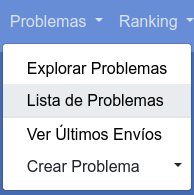
\includegraphics[width=.9\linewidth]{./ou_problem_bar.png}
        \end{minipage}\pause
        \begin{minipage}{.64\linewidth}
            Al hacer click en la pestaña de Problemas, podemos ver la lista de todos los problemas disponibles en el juez entrando a ``Lista de Problemas''.
        \end{minipage}
    \end{frame}

    \begin{frame}[noframenumbering]
        \begin{center}
            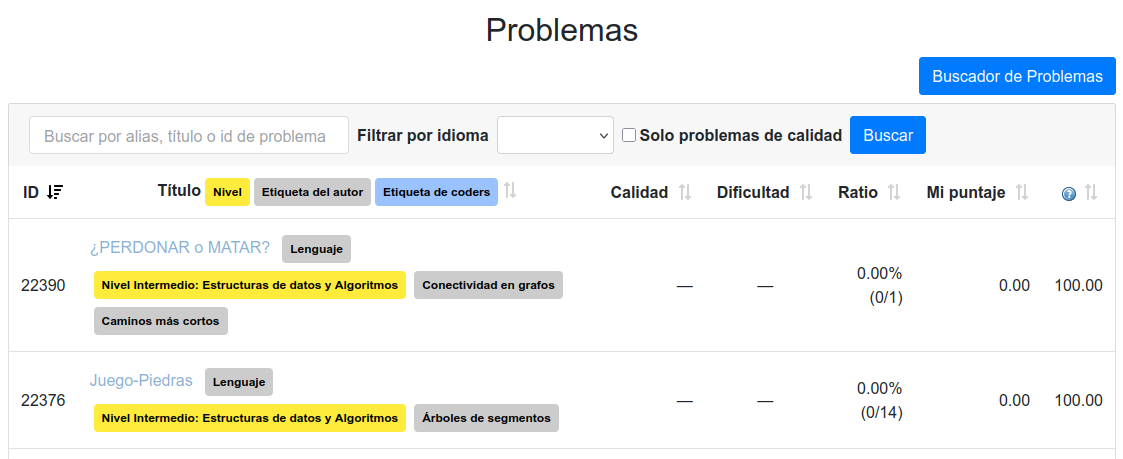
\includegraphics[width=.8\linewidth]{./ou_problems.png}\tikzmark{ou_problems}
        \end{center} \pause
        
        \begin{tikzpicture}[overlay, remember picture]
            \coordinate (a) at (pic cs:ou_problems);
            \uncover<3->{\draw[red, thick] ($ (a) + (-9.5,2.5) $) rectangle ($ (a) + (-9,.25) $);}
            \uncover<4->{
                \draw[blue, thick] ($ (a) + (-9.4,3) $) rectangle ($ (a) + (-6.6,2.55) $);
                \draw[blue, thick, ->] ($ (a) + (-1.15,2.8) $) -- ($ (a) + (-1.65,2.8) $);
            }
        \end{tikzpicture}

        Al ingresar al listado, nos encontraremos en una pantalla como esta. Los problemas al principio son los subidos más recientemente. \pause

        A la izquierda de cada problema aparece su \textbf{\textcolor{red}{id}}. Es muy común en los jueces online que cada problema tenga su id único. \pause

        En el caso de omegaUp, para buscar algún problema particular podemos usar el \textcolor{blue}{\textbf{buscador}} arriba ingresando su nombre (título) o su id, y haciendo click en ``Buscar''.
    \end{frame}

    \begin{frame}[noframenumbering]
        Si recordamos, ya habíamos visto un problema de omegaUp en la sección de complejidad... \pause probemos buscarlo por nombre en el buscador a ver si aparece. \pause

        \begin{center}
            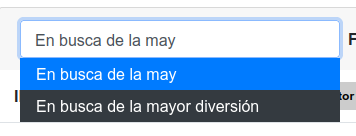
\includegraphics[width=.35\linewidth]{./ou_partial_search.png}
        \end{center} \pause

        Como es de esperarse, aparece listado incluso mientras escribimos su título. \pause

        \begin{center}
            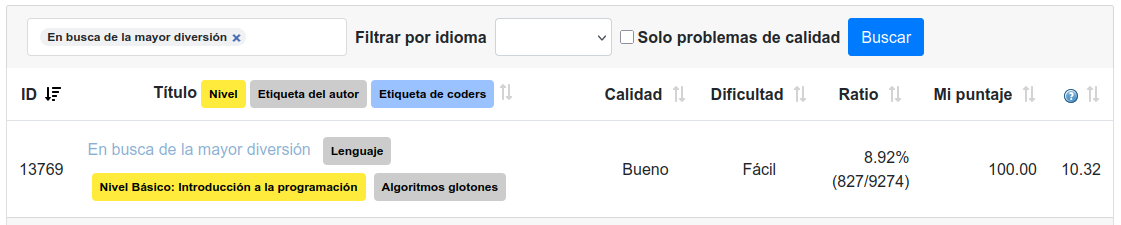
\includegraphics[width=\linewidth]{./ou_searched.png}
        \end{center} 
    \end{frame}

    \begin{frame}[noframenumbering]
        \begin{center}
            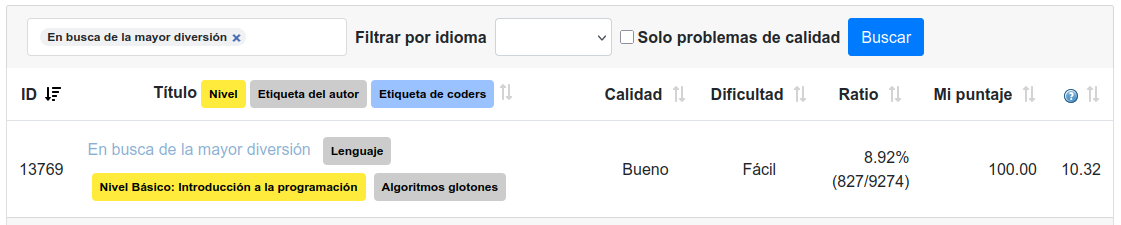
\includegraphics[width=\linewidth]{./ou_searched.png}\tikzmark{ou_searched}
        \end{center} \pause
        \begin{tikzpicture}[remember picture, overlay]
            \coordinate (a) at (pic cs:ou_searched);
            \uncover<8->{\draw[thick, Brown] ($ (a) + (-.75,1.6) $) rectangle ($ (a) + (-0.1,0.1) $);}
            \uncover<6->{\draw[thick, Purple] ($ (a) + (-2.1,1.6) $) rectangle ($ (a) + (-.8,0.1) $);}
            \uncover<5->{\draw[thick, ForestGreen] ($ (a) + (-3.25,1.6) $) rectangle ($ (a) + (-2.2,0.1) $);}
            \uncover<7->{\draw[thick, SkyBlue] ($ (a) + (-5.65,1.6) $) rectangle ($ (a) + (-3.35,0.1) $);}
            \uncover<3->{\draw[thick, Red] ($ (a) + (-8.1,0.625) $) rectangle ($ (a) + (-6.5,0.2) $);}
        \end{tikzpicture}\vspace{-18pt}

        Podemos identificar algunos detalles más que aparecen sobre el problema: \pause

        \begin{itemize}
            \item<3-> \textcolor{red}{\textbf{Técnicas / algoritmos relacionados con una posible solución}}.

            \uncover<4->{\textit{Esto puede spoilearnos la solución!} Muchos jueces permiten ocultar las etiquetas. En omegaUp ir a Mi perfil $\rightarrow$ Preferencias (o en \textcolor{blue}{\underline{\href{https://omegaup.com/profile/\#edit-preferences}{este link}}}).}

            \item<5->El \textcolor{ForestGreen}{\textbf{ratio}}: el porcentaje de envíos correctos respecto al total intentados por el resto de los usuarios de la página. Debajo nos indica \texttt{(aceptados / total)}.
            
            \item<6->\textbf{\textcolor{Purple}{Mi puntaje}}, el puntaje máximo obtenido en el problema. A mí me marca \texttt{100.00} porque ya lo resolví...

            \item<7->El \textbf{\textcolor{SkyBlue}{nivel de calidad y dificultad}} del problema. Poco común en otros jueces. Dado por votos de otros usuarios.

            \item<8->Un \textbf{\textcolor{Brown}{número de ranking}} de problema de omegaUp. No nos interesa mucho a nosotros.
        \end{itemize}
    \end{frame}

    \begin{frame}{Estructura de un problema}
        El formato de un problema depende de la competencia original donde se usó (si la hay) y/o del juez. \pause Entremos al enunciado del problema de antes y veamos los aspectos más importantes: \pause

        \begin{enumerate}
            \item \textbf{Título} / nombre del problema \pause
            \begin{center}
                \fbox{
                    
\includegraphics[width=.4\linewidth]{./ou_problem_title.png}
                }
            \end{center}\pause

        \item \textbf{Límite de tiempo} (por caso): \pause Cuando el programa es evaluado en el servidor, se lo suele ejecutar con ciertas entradas predefinidas llamados \textbf{casos de prueba} (salvo excepciones, ver ``problemas interactivos'') y se le da un cierto tiempo límite que puede tardar el programa en terminar de ejecutarse para cada entrada dada. \pause

            A este límite lo llamamos el \textit{límite de tiempo}, o en inglés, \textbf{time limit} (dado que muchos jueces online están en inglés), abreviado a veces \textit{TL}. \pause

            Es concretamente por este límite que es tan importante el análisis de complejidad de programas que vimos antes.

        \end{enumerate}
    \end{frame}

    \begin{frame}[noframenumbering]
        \begin{enumerate}
            \setcounter{enumi}{1}
            \item \textbf{Límite de tiempo} (por caso): (cont.) En el problema: \pause

            \begin{center}
                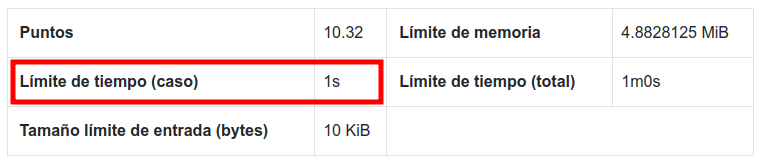
\includegraphics[width=.6\linewidth]{./ou_tl.png}
            \end{center} \pause

            En este problema, cada caso tiene un tiempo límite de 1s para ejecutarse. De lo contrario, la solución se considerará \textbf{incorrecta}. En breve veremos cómo el juez no comunica esto.

        \item \textbf{Límite de memoria} (por caso): \pause De forma análoga al time limit, existe el \textbf{memory limit} (a veces abreviado \textit{ML}) o \textit{límite de memoria}, que es la cantidad de memoria que el programa puede reservar durante la ejecución de cada caso de prueba. \pause En el problema: \pause
            \begin{center}
                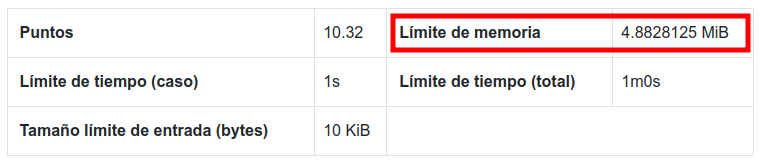
\includegraphics[width=.6\linewidth]{./ou_ml.png}
            \end{center} \pause

            Es decir, en este problema, al correr cada caso nuestra solución puede reservar a lo sumo 4.8828125 MiB. \pause Número raro...
        \end{enumerate}
    \end{frame}

    \begin{frame}[noframenumbering]
        \begin{enumerate}
            \setcounter{enumi}{3}
            \item \textbf{Descripción del problema}: \pause

            \begin{center}
                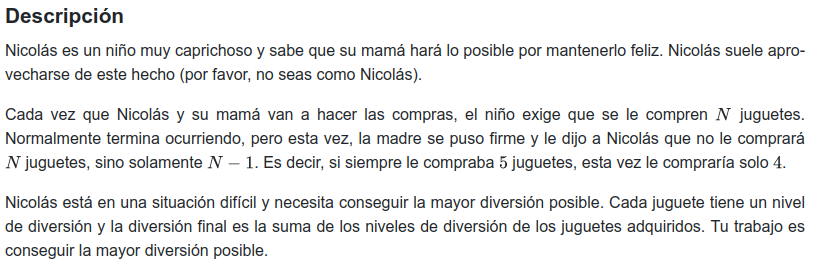
\includegraphics[width=.8\linewidth]{./ou_description.png}
            \end{center} \pause

        \item \textbf{Entrada}: \pause Suele incluir detalles específicos sobre cómo se provee la información del problema al programa que implementemos. \pause

            Dependiendo del juez / origen, también puede contener las \textbf{cotas} del problema, que en este caso se encuentran por separado más abajo. \pause

            \begin{center}
                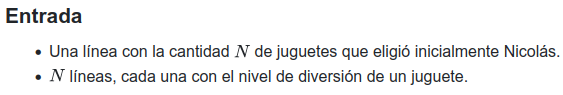
\includegraphics[width=.8\linewidth]{./ou_input.png}
            \end{center}
        \end{enumerate}
    \end{frame}

    \begin{frame}[noframenumbering]
        \begin{enumerate}
            \setcounter{enumi}{5}
            \item \textbf{Salida}: \pause De forma análoga a la entrada, especifica detalles sobre cómo escribir el resultado de resolver el problema para la entrada dada. En algunos casos presenta información más importante como ``qué solución imprimir'' si es que hay varias o qué imprimir si una solución ``no existe'' (según el problema). \pause

            \begin{center}
                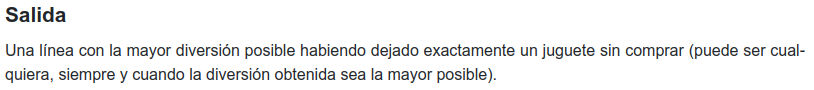
\includegraphics[width=.7\linewidth]{./ou_output.png}
            \end{center}\pause

        \item \textbf{Ejemplo(s)}: \pause Casi siempre los problemas contienen uno o más ejemplos (\textbf{samples}, en inglés) de entrada y salida válidos para una solución del problema, con el fin de comprender correctamente el formato de ambos o incluso aclarar el enunciado. \pause

            \begin{center}
                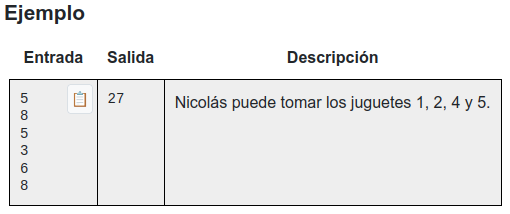
\includegraphics[width=.4\linewidth]{./ou_sample.png}
            \end{center}\pause

            En omegaUp también suelen incluir una \textit{Descripción} al lado de los ejemplos, explicando los resultados presentados. Otros jueces suelen incluir esto en una sección separada llamada \textit{Notas}. 
        \end{enumerate}
    \end{frame}

    \begin{frame}[noframenumbering]
        \begin{enumerate}
            \setcounter{enumi}{5}
            \item \textbf{Cotas}: \pause Establecen el intervalo o conjunto de valores que toman los valores de la entrada y/o la cantidad máxima de elementos que pueden haber en un caso de prueba. \pause 

            Son muy importantes junto con el límite de tiempo en cuanto a \textit{qué tan eficiente debe ser una solución} para resolver el problema. \pause 

            En efecto, según la cota asintótica superior de la solución, la cantidad de operaciones que realiza respecto a la entrada puede ser o no suficiente para correr en el tiempo límite establecido para el problema, y nuestra elección depende de qué sea ``más rápido'' (como cuando discutimos elegir selection vs merge sort).\pause
            \begin{center}
                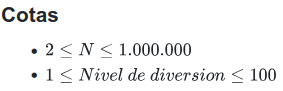
\includegraphics[width=.4\linewidth]{./ou_restrictions.png}
            \end{center}\pause

            En este caso, cada caso de prueba tiene a lo sumo $1,000,000 = 10^6$ números, cada uno con un valor entre $1$ y $100$.
        \end{enumerate}
    \end{frame}
 
    \begin{frame}[noframenumbering]
        \begin{enumerate}
            \setcounter{enumi}{6}
            \item \textbf{Subtareas}: Sólo existen en las competencias tipo ``IOI'' donde cada problema otorga hasta 100 puntos. Así, \textbf{no} hay subtareas en ICPC. \pause

                Establecen restricciones adicionales al enunciado original de forma que si se sube una solución correcta bajo la restricción agregada, otorgan \textbf{puntaje parcial}, una cantidad menor a 100 puntos indicado al lado de la subtarea. \pause

            \begin{center}
                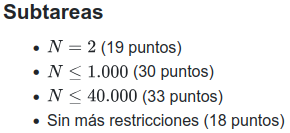
\includegraphics[width=.4\linewidth]{./ou_subtasks.png}
            \end{center}\pause

            Por ejemplo, para este problema, si lo resolvemos suponiendo que se dan \textbf{sólo dos números en la entrada} obtenemos 19 puntos. \pause De 100 puntos, 19 por algo sencillo no está mal, no? \pause

            ``Sin más restricciones'' indica los puntos otorgados por encima de las otras subtareas, es decir, puntos que sólo podríamos obtener si se resuelve el problema correctamente sin restricciones adicionales al enunciado original, como dice el nombre.
        \end{enumerate}
    \end{frame}

    \begin{frame}[noframenumbering]
        \begin{enumerate}
            \setcounter{enumi}{6}
            \item \textbf{Subtareas} (cont.): En competencias tipo IOI es muy importante prestar atención a las subtareas, porque nos permiten obtener puntaje sin encontrar la solución del problema sin restricciones, que puede ser significativamente más difícil de pensar e incluso implementar. \pause \vspace{4pt}

            La mayoría de jueces suelen contener más problemas tipo ICPC, es decir, que no incluyen subtareas. Más adelante mencionaremos qué jueces y en dónde contienen problemas de este tipo. \pause \vspace{4pt}

            Una última consideración a tener en cuenta parte de cómo se suman los puntajes de las subtareas. 
        \end{enumerate}
    \end{frame}

    \begin{frame}[noframenumbering]
        \begin{enumerate}
            \setcounter{enumi}{6}
            \item \textbf{Subtareas} (cont.): Hay dos formas usuales en las que se maneja la suma de los puntajes de las subtareas en las competencias y jueces online: \pause
                \begin{itemize}
                    \setlength\itemsep{.15em}
                    \item Una forma es que se puedan subir \textbf{múltiples soluciones} a un problema, y que se sumen los mejores puntajes por subtarea entre las distintas soluciones subidas \pause (por ejemplo, selectivo de OIA e IOI). \pause
                    \item Otra forma más clásica es que simplemente se tome el mayor puntaje entre todas las subidas, y que sea responsabilidad del competidor \textbf{detectar} la subtarea en función de la entrada en el código, a fin de ejecutar la solución correspondiente a la subtarea que hayamos pensado, y sumar los puntos respectivos \pause (por ejemplo, omegaUp, y en particular, el Torneo Jujeño de Programación). \pause
                \end{itemize}
            Idealmente deben consultar el reglamento de la competencia y el funcionamiento del juez en cada caso.
        \end{enumerate}
    \end{frame}

    \subsection{Veredictos}
    \begin{frame}
        \tableofcontents[currentsection, currentsubsection]
    \end{frame}

    \begin{frame}[fragile]{Probemos la solución que propusimos}
        Recordemos el enunciado y la solución propuesta al problema de antes:\pause

        \begin{block}{Problema (En busca de la mayor diversión, omegaUp 13769)}
            Nicolás quiere que le compren $N$ juguetes pero su mamá sólo le comprará $N-1$. El chico le asignó un nivel de diversión positivo a cada uno de los $N$ juguetes, dados por entrada. Queremos obtener la mayor diversión posible con $N-1$ juguetes de los $N$ dados.
        \end{block}

        \pause
        \begin{minted}[fontsize=\scriptsize]{cpp}
int n; cin >> n;
vector<int> arr(n);
for (int i = 0; i < n; i++) cin >> arr[i]; // Leemos los números

int sum = 0, mini = arr[0];
for (int i = 0; i < n; i++) // Obtenemos su suma y el mínimo entre ellos
    sum += arr[i], mini = min(mini, arr[i]);

cout << sum - mini << '\n'; // Imprimimos la suma restado el nro. más chico
        \end{minted}
        \pause

        \begin{center}
            \LARGE ¡Probemos subirlo al juez!
        \end{center}
    \end{frame}

    \begin{frame}{¿Y, juez?}
        \pause
        \begin{center}
            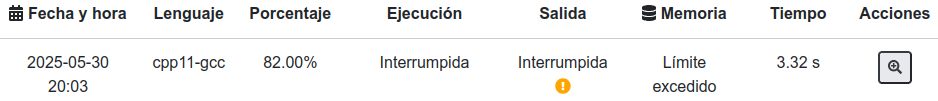
\includegraphics[width=.9\linewidth]{./ou_problem_mle.png}
        \end{center} \pause

        Nuestro primer veredicto! \pause Sacamos 82ptos (82\% del total en omegaUp), pero nos \textbf{excedimos del límite de memoria}. \pause 

        Si recordamos las subtareas, significa que obtuvimos \textit{puntaje parcial}, sumando puntos de todas las subtareas menos la última ``sin restricciones'':

        \begin{center}
            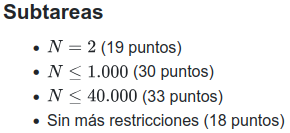
\includegraphics[width=.25\linewidth]{./ou_subtasks.png}
        \end{center}\pause

        Es decir, nuestro código es correcto para $N = 2$, para $N \leq 1000$ y para $N \leq 40000$. 
    \end{frame}

    \begin{frame}[noframenumbering]
        Se acuerdan que habíamos dicho que el problema tiene trampa? \pause Bueno, acá está: el límite de memoria es muy bajo. \pause Esto explica un poco el número raro que habíamos visto... \pause

        \begin{center}
            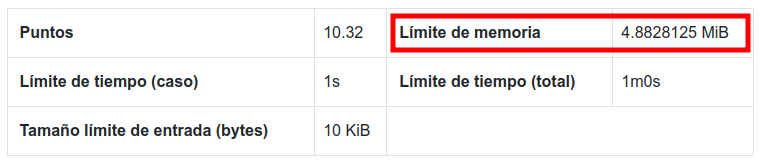
\includegraphics[width=.6\linewidth]{./ou_ml.png}
        \end{center} \pause

        Si bien nos enfocamos en esta clase en analizar cuánto tiempo tarda en correr una solución, podemos ver brevemente por qué nos pasamos del límite de memoria.
    \end{frame}

    \begin{frame}[noframenumbering]
        \setlength{\leftmargini}{12pt}
        \begin{itemize}
            \item Observemos que en la solución creamos un \mintinline{cpp}{vector<int>} de $N$ elementos. \pause Supongamos que nuestra solución ejecuta un caso con $N = 10^6$ números, la máxima posible según las cotas del problema (y una cantidad mayor a las subtareas donde sabemos que la solución es correcta). \pause

            \item Entonces, como cada \mintinline{cpp}{int} ocupa 32 bits (4 bytes), un \mintinline{cpp}{vector<int>} de $N = 10^6$ elementos ocupa alrededor de $4 \cdot 10^6$ bytes, o sea, $4 \cdot 10^6 / 1024 \approx 3906$ KiB (kibibytes), que son $3906 / 1024 \approx 3.8147$ MiB (mebibytes). \pause

            \item Si bien $3.8147$ MiB $<$ $4.8828125$ MiB, no son números muy lejanos entre sí, y un programa puede reservar algo de memoria adicional para funcionar correctamente (y también reservamos algunos \mintinline{cpp}{int} más, aunque el espacio que ocupan no es significante).
        \end{itemize} \pause

        Nos preguntamos entonces: ¿Existe una forma de usar menos memoria?
    \end{frame}

    \begin{frame}[fragile]{Una forma de usar menos memoria}
        \begin{block}{Observación}
            \pause
            Cada número de la entrada está entre 1 y 100 (recordar las cotas). \pause Como un byte puede almacenar números en el intervalo $[-128, 127]$, cada número entra en un byte. \pause Entonces, podemos reemplazar nuestro \mintinline{cpp}{vector<int>} con un \mintinline{cpp}{vector<char>}!
        \end{block} \pause

        Así, teniendo cuidado de hacer \textbf{casts} a \mintinline{cpp}{int} cuando sea necesario: \pause

        \begin{minted}[fontsize=\scriptsize]{cpp}
int n; cin >> n;
vector<char> arr(n);
for (int i = 0; i < n; i++) {int x; cin >> x; arr[i] = x;}

int sum = 0, mini = arr[0];
for (int i = 0; i < n; i++)
    sum += (int)arr[i], mini = min(mini, (int)arr[i]);

cout << sum - mini << '\n';
        \end{minted}

        \begin{center}
            \LARGE
            ¿Probamos de nuevo?
        \end{center}
    \end{frame}

    \begin{frame}[noframenumbering]
        \begin{center}
            
\includegraphics[width=16pt]{drumroll.png}
\includegraphics[width=16pt]{drumroll.png}
\includegraphics[width=16pt]{drumroll.png}
        \end{center} \pause

        \begin{center}
            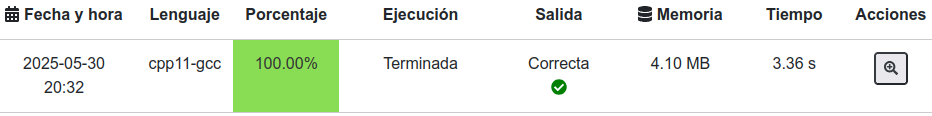
\includegraphics[width=.9\linewidth]{./ou_problem_ac_char.png}
        \end{center} \pause

        \textbf{\textcolor{green}{100 ptos}}! \pause Cuando nuestra solución es correcta (sin restricciones si el problema es tipo IOI), decimos que la solución fue \textit{\textcolor{green}{aceptada}}, o en inglés, \textbf{\textcolor{green}{Accepted}}, abreviado \textbf{\textcolor{green}{AC}}. \pause \vspace{4pt}

        Por otro lado, el veredicto que tuvimos inicialmente suele recibir el nombre de \textit{límite de memoria excedida}, o en inglés, \textbf{Memory Limit Exceeded}, abreviado normalmente como \textbf{MLE}. \pause

        Este veredicto no es tan común en IOI o OIA, porque el límite de memoria suele ser bastante alto, típicamente (aunque con excepciones) de 512 MiB, bastante más que los $\approx 4.8$ MiB de este problema. \pause 

        Más aún, no es demasiado común que el límite de memoria sea un factor importante en la solución del problema, muchas veces siendo más relevante el límite de tiempo. \pause Es más fácil ``alcanzar primero'' el límite de tiempo procesando tanta información, que el de memoria.
    \end{frame}

    \begin{frame}[noframenumbering]
        \begin{center}
            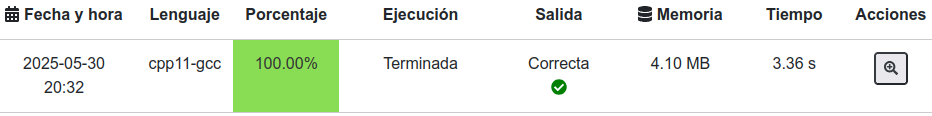
\includegraphics[width=.9\linewidth]{./ou_problem_ac_char.png}
        \end{center}

        Otra cosa importante a remarcar es el uso de memoria de nuestro programa: $4.10$ MiB. \pause Si bien calculando, nuestra solución debería reservar alrededor de $1 \cdot 10^6$ bytes para el \mintinline{cpp}{vector<char>} que usamos, o sea, $\approx 0.95$ MiB, la cantidad reportada por omegaUp es significativamente más alta. \pause Esto puede ser por diversos factores, como que \mintinline{cpp}{std::vector} almacena otro tipo de información que ocupa memoria, entre otros elementos del funcionamiento de nuestro programa en C++ que requieren reservar más memoria de la esperada. \pause

        Por este motivo, si obtenemos un veredicto \textbf{MLE}, debemos ser generosos en nuestra estimación de memoria utilizada, con el fin de tener cierto margen para que nuestra solución respete el límite de memoria del problema.
    \end{frame}

    \begin{frame}[fragile]{Otra forma de usar menos memoria}
        \pause
        \begin{block}{Observación}
            Se pueden procesar los números sin almacenarlos en un \mintinline{cpp}{std::vector}.
        \end{block} \pause
        En efecto, como sólo queremos obtener la suma y el mínimo del arreglo, directamente podemos procesarlos a medida se los lee desde la entrada, sin crear un arreglo para almacenar los enteros:\pause

        \begin{minted}[fontsize=\scriptsize]{cpp}
int n; cin >> n;
int sum = 0;
int mini = 150; // 150 es más grande que cualquier elem. de la entrada
for (int i = 0; i < n; i++) {
    int x; cin >> x;
    sum += x, mini = min(mini, x);
}
cout << sum - mini << '\n';
        \end{minted}
        \pause

        Cuando lo subimos al juez la solución es correcta y consume \textbf{aún menos} memoria: \pause
        \begin{center}
            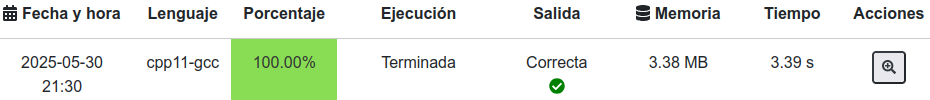
\includegraphics[width=.8\linewidth]{./ou_problem_ac_novec.png}
        \end{center}
    \end{frame}

    \begin{frame}{Seguimos recordando problemas...}
        El problema de antes no es el único que introdujimos en la sección de complejidad: \pause

        \begin{block}{Problema (Watermelon, CodeForces 4A)}
            Pete y Billy quieren dividir una sandía de peso $w$ kg en dos pedazos con peso \textbf{par}. Dado $w$, ¿es posible?
        \end{block} \pause

        El juez es otro ahora: \pause

        \begin{center}
            \href{https://codeforces.com/}{\includesvg[width=.6\linewidth]{cf_logo.svg}}
        \end{center} \pause 

        Es uno de los jueces más populares, con muchos problemas (tipo ICPC), competencias de alta calidad organizadas de forma regular y un sistema de rating. \pause \vspace{-4pt}

        \begin{center}
            \LARGE
            ¡Busquemos el problema en el juez!
        \end{center}
    \end{frame}

    \begin{frame}[noframenumbering]
        Identifiquemos lo importante: \pause
        \begin{itemize}
            \item \textbf{TL}: 1 segundo \pause
            \item \textbf{ML}: 64MB (acá son megabytes, no mebibytes) \pause
            \item \textbf{Enunciado}: Ya lo sabemos, la dada en la diapositiva anterior es una versión digerida del original. \pause
            \item \textbf{Entrada y Cotas}: Un entero $w$ con $1 \leq w \leq 100$. \pause
            \item \textbf{Salida}: Imprimir \texttt{YES} o \texttt{NO} según si se puede dividir la sandía. \pause
            \item \textbf{Ejemplo}: 
                \begin{center}
                    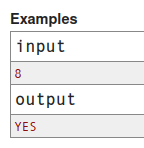
\includegraphics[height=.2\textheight]{./cf_example.png}
                \end{center} \pause
                Una explicación del ejemplo está en la sección \textit{Note}:

                \begin{center}
                    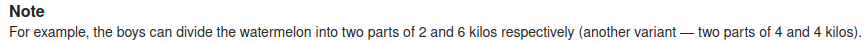
\includegraphics[width=.9\linewidth]{./cf_note.png}
                \end{center} \pause
            \item \textbf{Subtareas}: \textbf{No hay}, es estilo ICPC.
        \end{itemize}
    \end{frame}

    \begin{frame}[fragile]{Otra solución con un problema}
        Recordemos la solución que propusimos al problema: \pause

        \begin{minted}[fontsize=\small]{cpp}
int w; cin >> w;
if ((w%2) == 0)
    cout << "YES"; 
else
    cout << "NO"; 
        \end{minted}
        \pause

        \begin{center}
            \LARGE
            ¡Probemos subirlo al juez!
        \end{center} \pause

        \begin{center}
            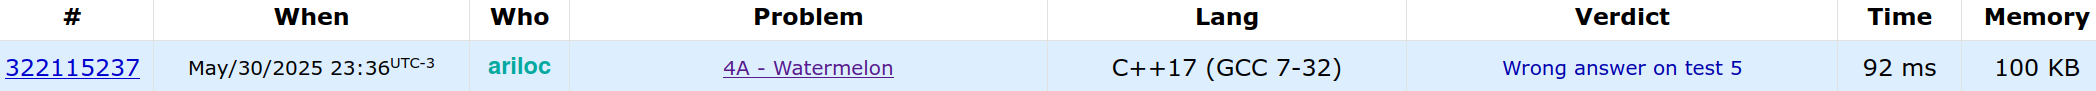
\includegraphics[width=.95\linewidth]{./cf_wa.png}
        \end{center}\pause

        Obtuvimos un nuevo veredicto: \textbf{\textcolor{red}{Wrong Answer}} (abreviado como \textbf{\textcolor{red}{WA}}), es decir, \textit{\textcolor{red}{respuesta incorrecta}}. \pause

        Esto significa que nuestra solución es incorrecta, pero no porque hayamos excedido algún límite, sino porque nuestra solución en algún caso de prueba imprime una respuesta que \textbf{no es correcta} según el enunciado.
    \end{frame}

    \begin{frame}[noframenumbering]
        Un \textcolor{red}{Wrong Answer} es uno de los veredictos más comunes. Nuestra solución puede estar imprimiendo una respuesta incorrecta por uno (o ambos) de dos motivos principales: \pause

        \begin{itemize}
            \item La solución que pensamos al problema es incorrecta, no lo resuelve siempre. \pause

            \item Nuestra implementación de la solución tiene un error, un \textbf{bug}, que hace que no represente la idea que queremos reflejar en código. \pause
        \end{itemize}

        Por supuesto, hay variantes a estos motivos. Hay casos donde la idea está ``casi bien'', y capaz nos falta considerar un caso muy específico en nuestro código, por ejemplo para entradas muy chicas ($n=0$, $n=1$, etc, si el problema lo permite). A este tipo de casos los conocemos como \textbf{casos borde}. \pause

        Curiosamente, es precisamente un caso borde lo que hace que nuestra solución al problema anterior falle.
    \end{frame}

    \begin{frame}[noframenumbering]
        Pensemos por un momento: ¿basta sólo con que el peso de la sandía sea par para poder dividirla en dos pedazos pares? \pause

        Dedujimos esto porque vimos que si es posible, como la suma de dos núemros pares es par, entonces $w$ debe ser par. Pero esto no implica que sea al revés.\pause

        En efecto, sabemos que $1 \leq w \leq 100$, entonces $w = 2$ es una posible entrada a nuestro programa: \pause
            \begin{itemize}
                \item $w = 2$ es par, entonces nuestra solución anterior imprimiría que la sandía \textbf{sí} se puede dividir en dos pedazos pares.\pause
                \item Sin embargo, la única forma de dividir la sandía en dos partes con peso \textit{entero} es que ambas pesen $1$kg, por lo que \textbf{no} se la puede dividir en pedazos de peso par.\pause
            \end{itemize}

        Encontramos nuestro caso borde! \pause ¿Pero cómo lo resolvemos? ¿Es el único caso donde nuestra solución estaba mal?
    \end{frame}

    \begin{frame}[fragile]{En busca de otro \textbf{AC}}
        Analicemos lo que sabemos: \pause
        \begin{itemize}
            \item $w$ \textbf{tiene} que ser par para que la respuesta sea \texttt{YES}. \pause
            \item Si $w=2$, la respuesta es \texttt{NO}. \pause
        \end{itemize}

        Así, veamos que si $w>2$ y $w$ par, la respuesta es siempre \texttt{YES}. \pause 

        Esto se debe a que, si $w$ cumple las condiciones, en particular $w \geq 4$, entonces se puede dividir a $w$ en un pedazo de peso $2$kg, y otro de peso $(w-2)$kg, que será positivo y par porque restamos dos números pares. \pause

        De esta forma, sólo debemos cubrir el caso borde mencionado en la solución antes presentada: \pause \vspace{4pt}

        \begin{minipage}{.49\linewidth}
        \begin{minted}[fontsize=\scriptsize]{cpp}
int w; cin >> w;
if ((w%2) == 0 && w != 2)
    cout << "YES";
else
    cout << "NO";
        \end{minted}
        \end{minipage}\pause
        \begin{minipage}{.49\linewidth}
        \begin{center}
            \LARGE
            ¿Probamos de nuevo?
        \end{center}
        \end{minipage}
        \pause

        \begin{center}
            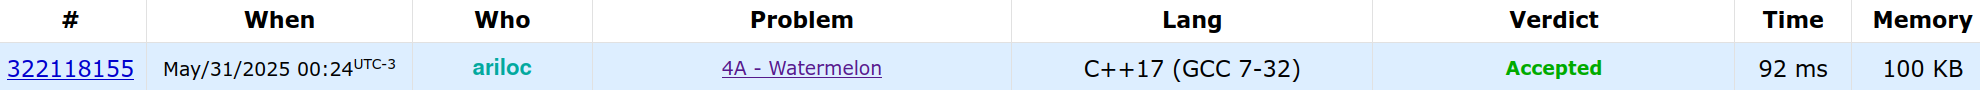
\includegraphics[width=.95\linewidth]{./cf_ac.png}
        \end{center}
    \end{frame}

    \begin{frame}{Un juez más, y no podemos más!}
        Tanto decir que es importante que nuestro programa vaya rápido, veamos ahora cómo el juez nos informa que nuestro programa excedió el \textit{límite de tiempo del problema}. Para ello, aprovechemos otro problema más que introdujimos antes: \pause

        \begin{block}{Problema (Nearest Smaller Values, CSES 1645)}
            Dado un arreglo de $n$ enteros, encontrar para cada posición del arreglo la posición más cercana a su izquierda que tenga un menor valor a la primera. $1 \leq n \leq 2 \cdot 10^5$
        \end{block} \pause

        Otro juez más:\pause
        \begin{center}
            \href{https://cses.fi/}{
\includegraphics[width=.4\linewidth]{cses_logo.png}}
        \end{center} 
    \end{frame}

    \begin{frame}[noframenumbering]
        \begin{center}
            \href{https://cses.fi/}{
\includegraphics[width=.4\linewidth]{cses_logo.png}}
        \end{center} \pause

        Es un juez utilizado en Finlandia para organizar competencias que tiene un conjunto de problemas reducido pero de muy buena calidad, orientados a educar en diversos temas de Programación Competitiva. \pause \vspace{4pt}

        Uno de sus principales desarrolladores es Antti Laaksonen, escritor del libro ``\textit{Guide To Competitive Programming}''. Muchos de los problemas y soluciones que describe en el libro pueden resolverse en CSES. \pause

        \begin{center}
            \LARGE
            ¡Busquemos el problema en el juez!
        \end{center}
    \end{frame}

    \begin{frame}[noframenumbering]
        No es problema identificar las partes del problema en CSES. \pause 

        Lo que más nos interesa es que el \textbf{TL} es 1s, y el \textbf{ML} es 512MB, números muy comunes para problemas de Programación Competitiva. \pause 

        Además no hay subtareas, es estilo ICPC. \pause \vspace{4pt}

        En la sección de análisis amortizado (\textit{si no la salteamos por tiempo}) vimos una solución en $\mathcal{O}(n)$ que resuelve este problema. Dicha solución es correcta y mandarla al juez resulta en un veredicto \textbf{\textcolor{green}{Accepted}}, se los prometo. \pause

        Lo que nos vamos a enfocar es ver qué pasa si mandamos una solución que es muy lenta, como una que corre en $\mathcal{O}(n^2)$. 
    \end{frame}

    \begin{frame}[fragile]{Cuando nos pasamos de tiempo}
        Proponemos la siguiente solución ``ingenua'' o \textit{naive} al problema, que corre en $\mathcal{O}(n^2)$: \pause \vspace{4pt}
    
    \begin{minted}[fontsize=\scriptsize]{cpp}
vector<int> arr(n);
for (int i = 0; i < n; i++)
    cin >> arr[i];

for (int i = 0; i < n; i++) {
    int nsv = -1;
    for (int j = i-1; j >= 0 && nsv == -1; j--)
        if (arr[j] < arr[i])
            nsv = j;
    cout << nsv+1 << ' ';
}
    \end{minted}
    \pause

        Siendo $1 \leq n \leq 2 \cdot 10^5$, la cantidad de operaciones que ejecuta una solución con una cota asintótica tal supera ampliamente el rule of thumb que conocemos para que el programa termine en 1s. \pause

    \begin{center}
        \LARGE
        ¡Probemos subirlo al juez!
    \end{center}
    \end{frame}

    \begin{frame}[noframenumbering]
        \begin{center}
            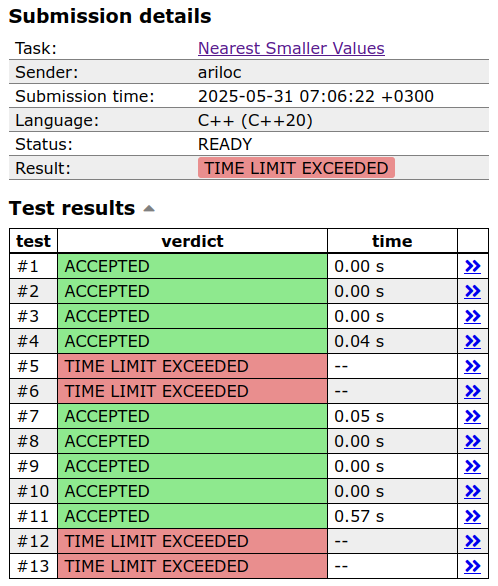
\includegraphics[width=.4\linewidth]{./cses_tle.png}
        \end{center}
        \pause

        Nuevo veredicto adquirido: \textbf{Time Limit Exceeded} (abreviado normalmente como \textbf{TLE}), o en español, \textit{tiempo límite excedido}. Como dice su nombre, nos indica que en al menos uno de los casos nuestra solución tardó más de 1s en ejecutarse para la entrada dada.
    \end{frame}

    \begin{frame}[noframenumbering]
        A diferencia de CodeForces donde sólo se ejecutan los casos en orden y se detiene la ejecución apenas falla en alguno, en CSES se ejecutan todos los casos sin importar si alguno ``anterior'' falló. \pause Más aún, se pueden ver y descargar los casos para verlos e intentar resolver los problemas en nuestro código. \pause \textbf{NO hay que acostumbrarse a esto}, en las competencias \textbf{NO} podemos ver los casos de prueba, y tampoco en muchos jueces: \pause

        \begin{itemize}
            \item omegaUp nunca deja ver los casos, y a veces tampoco qué subtareas funcionaron, a menos que se haya resuelto el problema antes con 100ptos. \pause
            \item CodeForces deja ver los casos de prueba sólo en modo práctica (no en competencia), e incluso así están recortados, impidiendo ver la totalidad de casos grandes.\pause
            \item El \textbf{OIA Juez} nunca deja ver los casos, aunque sí las subtareas, sus puntajes correspondientes al total obtenido, e incluso a veces el veredicto obtenido en los casos de la subtarea.
        \end{itemize}
    \end{frame}

    \begin{frame}{Un último veredicto no menos importante}
        Finalmente, vamos a introducir un último veredicto no menos importante a los ya vistos: el \textbf{Runtime Error} (abreviado \textbf{RE} o \textbf{RTE}), o en español, \textit{error de ejecución}. \pause

        ¿Alguna vez les pasó que ejecutaron un programa en C++ y terminó abruptamente con \texttt{Segmentation fault (core dumped)}? \pause Si nuestro programa ``crashea'' ejecutando algún caso en el juez, el veredicto mostrado será entonces \textit{Runtime Error}. \vspace{4pt} \pause

        El origen de un error de este tipo es claramente por un problema en la implementación de la solución, un bug en la programación. El más común de estos errores es ``acceder a una posición fuera de memoria'', por ejemplo, tener un \mintinline{cpp}{vector<int>} con tamaño $n$ y querer acceder/escribir en algún punto a \texttt{arr[n]} (inválido porque está indexado en 0), o a \texttt{arr[-1]}.
    \end{frame}

    \begin{frame}{\textbf{RE} en algunos jueces}
        A veces los runtime error no están marcados de forma clara en los jueces. Presentamos algunos ejemplos para que sepan identificarlos:\pause
        \setlength{\leftmargini}{16pt}
        \begin{itemize}
            \item \textbf{omegaUp}: ``Error de ejecución''
            \begin{center}
                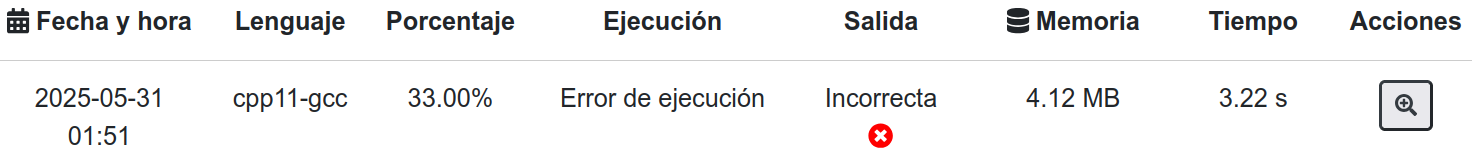
\includegraphics[width=.8\linewidth]{./ou_rte.png}
            \end{center}

            \item \textbf{CodeForces}: ``Runtime error on test ...''
            \begin{center}
                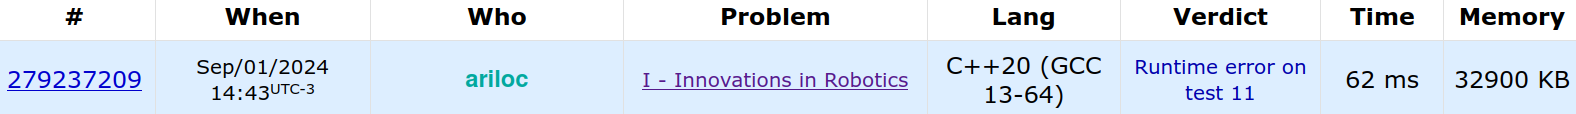
\includegraphics[width=.8\linewidth]{./cf_rte.png}
            \end{center}
            
            \item \textbf{OIA Juez}: ``Execution killed (could be triggered by violating memory limits)''
            \begin{center}
                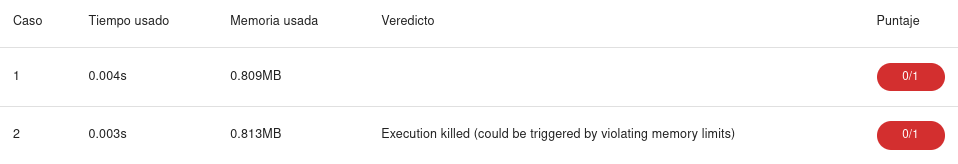
\includegraphics[width=.8\linewidth]{./oiaj_rte.png}
            \end{center}

            \item \textbf{SPOJ}: ``runtime error (SIGSEGV)''
            \begin{center}
                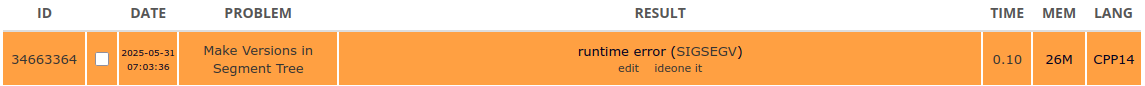
\includegraphics[width=.8\linewidth]{./spoj_rte.png}
            \end{center}
        \item 
        \end{itemize}
    \end{frame}

    \begin{frame}{Recapitulando}
        Tenemos entonces los siguientes veredictos principales posibles: \pause

        \begin{itemize}
            \item \textbf{\textcolor{green}{Accepted}}: Nuestra solución resuelve todos los casos de prueba correctamente y en los límites estipulados.\pause
            \item \textbf{TLE}: Nuestra solución excede el límite de \textit{tiempo} estipulado en algún caso de prueba.\pause

            \item \textbf{MLE}: Nuestra solución excede el límite de \textit{memoria} estipulado en algún caso de prueba.\pause

            \item \textbf{\textcolor{red}{WA}}: Nuestra solución no excede ninguno de los límites estipulados, pero escribe una respuesta incorrecta en alguno de los casos de prueba. \pause
        \end{itemize}

        Y además, en problemas tipo IOI, los problemas pueden tener puntaje parcial, donde cada subtarea tiene su propio veredicto, y las subtareas \textbf{\textcolor{green}{AC}} otorgan puntos según sea indicado. El veredicto general que se muestra depende del juez, pero no tomará \textbf{\textcolor{green}{AC}} si no todas las subtareas son \textbf{\textcolor{green}{AC}}.
    \end{frame}

    \begin{frame}
        \begin{alertblock}{$\mathcal{O}$J$\mathcal{O}$!}
            \pause
            En algunos casos también las subtareas pueden tener puntaje parcial. Por ejemplo, el enunciado puede consistir en imprimir dos líneas, una con un resultado y otra con ``una forma de obtener ese resultado'' (según el contexto del problema), y se indica algo como que ``Se otorga el 50\% del puntaje si se imprime correctamente la primer línea, y el 50\% restante si se imprime correctamente la segunda''. \pause \vspace{4pt}

            En estos casos hay que prestar atención al enunciado, pero indica que también puede haber puntaje parcial más allá de las subtareas. Es decir, si el enunciado tiene un mensaje como el ejemplo anterior, suele pasar que el puntaje de cada subtarea se divide a la mitad, donde se otorga cada mitad del puntaje \textit{de la subtarea} según las líneas que se hayan impreso correctamente. 

            Por supuesto, hay que ver cada caso y leer el reglamento de la competencia (por ejemplo OIA).
        \end{alertblock}
    \end{frame}


    \subsection{omegaUp: competencias}
    \begin{frame}
        \tableofcontents[currentsection, currentsubsection]
    \end{frame}

    \begin{frame}{Competencias (concursos)}
        Previamente mencionamos que omegaUp permite crear competencias (llamados \textit{concursos}) fácilmente. \pause Probemos buscar un concurso. \vspace{8pt} \pause

        \begin{minipage}{.35\linewidth}
            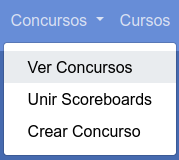
\includegraphics[width=.9\linewidth]{./ou_contest_bar.png}
        \end{minipage}\pause
        \begin{minipage}{.64\linewidth}
            Al hacer click en la pestaña Concursos desde la página principal, podemos ver la lista de todos los concursos disponibles entrando a ``Ver Concursos''.
        \end{minipage}
    \end{frame}

    \begin{frame}[noframenumbering]
        \begin{center}
            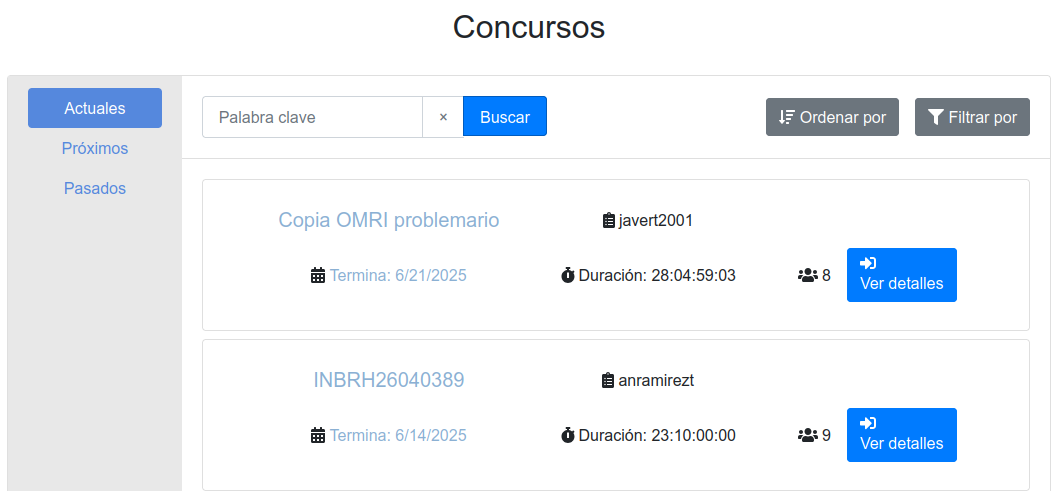
\includegraphics[width=.8\linewidth]{./ou_contests.png}
        \end{center}\pause
        Al ingresar, nos encontraremos en una pantalla como esta. Aquí se encuentran las competencias en curso, ordenadas por tiempo de finalización de ``más tarde a más temprano''. Hay que considerar que una competencia se puede armar para que dure días o incluso meses. \pause

        Como podemos ver, hay muchas competencias no relacionadas creadas por usuarios del sitio, en muchos casos para sus propios propósitos. \pause Dependiendo la competencia, también puede requerirse aprobación del autor para participar (por ejemplo, para la OII).
    \end{frame}

    \begin{frame}[noframenumbering]
        \begin{center}
            \LARGE
            ¡Entremos a un concurso y mostremos cómo funciona!
        \end{center}
    \end{frame}
    
    \subsection{Otros jueces}
    \begin{frame}
        \tableofcontents[currentsection, currentsubsection]
    \end{frame}

    \begin{frame}{Hay para elegir}
        Como habrán visto, hay muchísimos jueces para elegir. Además de los ya presentados, recomendamos también los siguientes, donde algunos ya los mencionamos: \pause

        \begin{itemize}
            \item \textbf{\textcolor{blue}{\href{https://juez.oia.unsam.edu.ar/}{OIA Juez}}}: Contiene problemas tipo IOI de las distintas instancias de la Olimpíada Informática Argentina de distintos años (Prog. Competitiva nivel secundario). Tiene muchos problemas muy buenos, incluyendo algunos interesantes para arrancar. Personalmente recomendado. \pause

            \item \textbf{\textcolor{blue}{\href{https://codeforces.com/gyms}{CodeForces Gym}}}: Además del set de problemas normal de CodeForces, la sección de ``Gym'' contiene, de forma similar a omegaUp, competencias subidas por los usuarios. Muchas de éstas incluyen copias de instancias regionales ICPC (Prog. Competitiva nivel universitario) de todo el mundo, incluyendo World Finals, siendo un recurso valiosísimo para entrenar en equipo.
        \end{itemize}
    \end{frame}

    \begin{frame}[noframenumbering]
        \begin{itemize}
            \item \textbf{\textcolor{blue}{\href{https://onlinejudge.org/}{UVa Online Judge}}}: Juez de antaño que data desde antes del año 2000. Contiene problemas de ICPC antiguos y un set de problemas diversos muy extenso. Muchos de sus problemas y soluciones están mencionados en la famosa serie de libros ``Competitive Programming'', de Steven y Felix Halim. \pause

            \item \textbf{\textcolor{blue}{\href{https://open.kattis.com/}{Kattis}}}: Un juez más reciente con algunos problemas interesantes, también citado por Steven y Felix Halim en su edición más reciente de su serie de libros de programación competititva, el ``Competitive Programming 4''.
        \end{itemize}
    \end{frame}

    \begin{frame}{Otros otros jueces}
        También mencionamos algunos jueces más con los cuales se pueden encontrar algún que otro problema de calidad, o problemas clásicos conocidos: \pause

        \begin{itemize}
            \item \textbf{\textcolor{blue}{\href{https://www.spoj.com/}{Sphere Online Judge (SPOJ)}}}: Conocido por problemas clásicos como DQUERY o KQUERY, al igual que algunos problemas viejos de instancias de ICPC de la UBA.
            \item \textbf{\textcolor{blue}{\href{https://www.hackerrank.com/contests}{HackerRank}}}: Conocido por su facilidad para armar contests, pueden encontrárselo alguna vez para competencias con problemas personalizados.
            \item \textbf{\textcolor{blue}{\href{https://atcoder.jp/}{AtCoder}}}: Juez de origen japonés con competencias regulares los sábados o domingos a la mañana (hora Argentina). Suele contener problemas distintos a otros lugares y algo creativos, con algunos problemas sencillos pero que suben de dificultad rápidamente.
        \end{itemize}
    \end{frame}

    \begin{frame}[noframenumbering]
        \begin{itemize}
            \item \textbf{\textcolor{blue}{\href{https://dmoj.ca/}{DMOJ}}}: Conocido por contener problemas de algunas IOIs viejas.
            \item \textbf{\textcolor{blue}{\href{https://oj.uz/problems}{oj.uz}}}: Conocido por contener problemas de distintas instancias regionales de competencias tipo IOI, incluyendo IOIs viejas.
            \item \textbf{\textcolor{blue}{\href{https://www.facebook.com/codingcompetitions/hacker-cup/2019}{Meta Hacker Cup}}}: Meta (Facebook) lleva a cabo una competencia de programación competitiva todos los años con problemas interesantes. Consultar el registro de problemas de años anteriores puede ser entretenido.
        \end{itemize}
    \end{frame}

    \begin{frame}{Comodín}
        También puede ser útil usar herramientas como \textbf{\textcolor{blue}{\href{https://vjudge.net/}{vJudge}}}, que recopilan problemas de múltiples jueces online, y permite crear competencias personalizadas con problemas de distintas fuentes.
    \end{frame}

    \section{Cierre}
    \begin{frame}
        \tableofcontents[currentsection]
    \end{frame}

    \begin{frame}
        \begin{center}
            \LARGE
            ¿Preguntas? ¿Dudas?
        \end{center}
    \end{frame}

    \begin{frame}
        \begin{center}
            \Huge
            ¡Muchas gracias!
        \end{center}
    \end{frame}

\end{document}
